%%%%%%%%%%%%%%%%%%%%%%%%%%%%%%%%%%%%%%%%%%%%%%%%%%%%%%%%%%%%%%%%%
%
%   Template para monografia de TCC-2018 - versao 1.0.alfa
%
%%%%%%%%%%%%%%%%%%%%%%%%%%%%%%%%%%%%%%%%%%%%%%%%%%%%%%%%%%%%%%%%%
%%
%% Este template utiliza o modelo mantido pela abnt e foi baseado 
%% no abtex2-modelo-trabalho-academico.tex, v-1.9.6 laurocesar
%% Copyright 2012-2016 by abnTeX2 group at http://www.abntex.net.br/ 
%%
% -------------------------------------------------------------------
%% This work may be distributed and/or modified under the conditions 
%% of the LaTeX Project Public License, either version 1.3 of this 
%% license or (at your option) any later version. The latest version 
%% of this license is in http://www.latex-project.org/lppl.txt
%% and version 1.3 or later is part of all distributions of LaTeX
%% version 2005/12/01 or later.
%%
%% This work has the LPPL maintenance status `maintained'.
%% 
%% The Current Maintainer of this work is the abnTeX2 team, led
%% by Lauro César Araujo. Further information are available on 
%% http://www.abntex.net.br/
%%
%% This work consists of the files abntex2-modelo-trabalho-academico.tex,
%% abntex2-modelo-include-comandos and abntex2-modelo-references.bib
% -------------------------------------------------------------------
%%
%% Modelo de Monografia em conformidade com ABNT NBR 14724:2011
%%
%%%%%%%%%%%%%%%%%%%%%%%%%%%%%%%%%%%%%%%%%%%%%%%%%%%%%%%%%%%%%%%%%
%%
%% ATENÇAO para as opções:
%%
%% para modo rascunho, sem páginas brancas, use: 
%% openany, oneside, nopartblankpage
%%
%% para modo normal, com tudo que ABNT exige, use:  
%% openright, twoside, partpageblank
%%

\documentclass[
	% -- opções da classe memoir --
	12pt,			% tamanho da fonte
	openany,		% capítulos começam em qq página (isso elimina várias pág brancas)
	%openright,		% capítulos começam em pág ímpar (insere página vazia caso preciso)
	oneside,		% considera impressão de um só lado (gera menos pág brancas)
	%twoside,		% para impressão em recto e verso. Oposto a oneside
	a4paper,		% tamanho do papel. 
	% -- opções da classe abntex2 --
	%chapter=TITLE,		% títulos de capítulos convertidos em letras maiúsculas
	%section=TITLE,		% títulos de seções convertidos em letras maiúsculas
	%subsection=TITLE,	% títulos de subseções convertidos em letras maiúsculas
	%subsubsection=TITLE,% títulos de subsubseções convertidos em letras maiúsculas
	% -- opções do pacote babel --
	english,		% idioma adicional para hifenização
	%french,		% idioma adicional para hifenização
	%spanish,		% idioma adicional para hifenização
	%portuges		% o último idioma é o principal do documento
	brazil			% o último idioma é o principal do documento
	]{abntex2}

\usepackage{graphicx}
\usepackage{pgfgantt}
\usepackage{pdfpages}
\usepackage[alf]{abntex2cite}
\usepackage{listings}
\usepackage{customize}
% ------------------------------------------------------------------------
%   Componente do template para monografia de TCC-2018 - versao 1.0.alfa
% ------------------------------------------------------------------------

%------------ Pacotes básicos 
\usepackage{lmodern}			% Usa a fonte Latin Modern			
\usepackage[T1]{fontenc}		% Selecao de codigos de fonte.
\usepackage[utf8]{inputenc}		% Codificacao do documento (conversão automática dos acentos)
\usepackage{lastpage}			% Usado pela Ficha catalográfica
\usepackage{indentfirst}		% Indenta o primeiro parágrafo de cada seção.
\usepackage{color}			% Controle das cores
\usepackage{graphicx}			% Inclusão de gráficos
\usepackage{microtype} 			% para melhorias de justificação
\usepackage{tabulary}
\usepackage{float}
\usepackage{url}
\usepackage{pgfgantt}
\usepackage{tikz}

% ----------------------------------------------------------
\usepackage{customize}
% ----------------------------------------------------------

%------------ Pacotes adicionais
\usepackage{blindtext}			% para geração de dummy text

%------------ Pacotes de citações
% \usepackage[backend=biber,style=numeric]{biblatex}
\usepackage[brazilian,hyperpageref]{backref}	% Paginas com as citações na bibl
\usepackage{abntex2cite}		% Citações padrão ABNT
\usepackage{pdfpages}			% Saida em pdf

%------------ Comandos úteis
\newcommand{\aspas}[1]{``#1''}

% ----------- CONFIGURAÇÕES DE PACOTES

% Configurações do pacote backref
% Usado sem a opção hyperpageref de backref
\renewcommand{\backrefpagesname}{Citado na(s) página(s):~}
% Texto padrão antes do número das páginas
\renewcommand{\backref}{}
% Define os textos da citação
\renewcommand*{\backrefalt}[4]{
	\ifcase #1 %
		Nenhuma citação no texto.%
	\or
		Citado na página #2.%
	\else
		Citado #1 vezes nas páginas #2.%
	\fi}%
% ---

% Espaçamentos entre linhas e parágrafos 
% O tamanho do parágrafo é dado por:
\setlength{\parindent}{1.3cm}
% Controle do espaçamento entre um parágrafo e outro:
\setlength{\parskip}{0.2cm}  % tente também \onelineskip

% compila o indice
\makeindex

% ----------------------------------------------------
% Configurações de aparência do PDF final
% ----------------------------------------------------

% alterando o aspecto da cor azul
\definecolor{blue}{RGB}{41,5,195}

% informações do PDF
\makeatletter
\hypersetup{
     	%pagebackref=true,
		pdftitle={\@title}, 
		pdfauthor={\@author},
    	pdfsubject={\imprimirpreambulo},
	    pdfcreator={LaTeX with abnTeX2},
		pdfkeywords={abnt}{latex}{abntex}{abntex2}{trabalho acadêmico}, 
		colorlinks=true,       		% false: boxed links; true: colored links
    	linkcolor=blue,          	% color of internal links
    	citecolor=blue,        		% color of links to bibliography
    	filecolor=magenta,      		% color of file links
		urlcolor=blue,
		bookmarksdepth=4
}
\makeatother

% ----------------------------------------------------
% Comandos para geração de itens textuais 
% ----------------------------------------------------

\newcommand{\imprimirfichacatalografica}{

\begin{fichacatalografica}
	\sffamily
	\vspace*{\fill}					% Posição vertical
	\begin{center}					% Minipage Centralizado
	\fbox{\begin{minipage}[c][8cm]{13.5cm}		% Largura
	\small
	
	\hspace{1cm} \imprimirautor\\

	\begingroup
        \leftskip4em
        \rightskip\leftskip
	
	\imprimirtitulo  / \imprimirautor. -- \imprimirlocal, \imprimirdata.
	
	\pageref{LastPage} p. : il. (algumas color.) ; 30 cm.\\
	
	\imprimirorientadorRotulo~\imprimirorientador\\
	
	%\imprimirtipotrabalho~--~\imprimirinstituicao, \imprimirdata.\\
	Monografia para trabalho de conclusão de curso (graduação)~--~Instituto Federal 
	de Educação, Ciência e Tecnologia de Minas Gerais, Ciência da Computação, 
	Formiga, \imprimirdata.\\
	
	1. Palavra-chave1.
	2. Palavra-chave2.
	3. Palavra-chave3.
	I. \imprimirorientador.
	II. Instituto Federal de Educação, Ciência e Tecnologia de Minas Gerais.
	III. Ciência da Computação.
	IV. \imprimirtitulo 			
        \par
        \endgroup
	\end{minipage}}
	\end{center}
\end{fichacatalografica}

}

\newcommand{\imprimirerrata}{

\begin{errata}
Exemplo de errata\\[1cm]

FERRIGNO, C. R. A. \textbf{Tratamento de neoplasias ósseas apendiculares com
reimplantação de enxerto ósseo autólogo autoclavado associado ao plasma
rico em plaquetas}: estudo crítico na cirurgia de preservação de membro em
cães. 2011. 128 f. Tese (Livre-Docência) - Faculdade de Medicina Veterinária e
Zootecnia, Universidade de São Paulo, São Paulo, 2011.

\begin{table}[htb]
\center
\footnotesize
\begin{tabular}{|p{1.4cm}|p{1cm}|p{3cm}|p{3cm}|}
  \hline
   \textbf{Folha} & \textbf{Linha}  & \textbf{Onde se lê}  & \textbf{Leia-se}  \\
    \hline
    1 & 10 & auto-conclavo & autoconclavo\\
   \hline
\end{tabular}
\end{table}

\end{errata}

}

\newcommand{\imprimirfolhadeaprovacao}[1]{

\begin{folhadeaprovacao}
  \begin{center}
   {\ABNTEXchapterfont\large\imprimirautor}

   \vspace*{\fill}\vspace*{\fill}
   \begin{center}
     \ABNTEXchapterfont\bfseries\Large\imprimirtitulo
   \end{center}
   \vspace*{\fill}
    
   \hspace{.45\textwidth}
   \begin{minipage}{.5\textwidth}
       \imprimirpreambulo
   \end{minipage}%
   \vspace*{\fill}        
   \end{center}
   
   Trabalho aprovado em {#1}.
   
   \vspace{1cm}
   \hspace{4cm} BANCA EXAMINADORA    

   \assinatura{\textbf{\imprimirorientador} \\ Orientador} 
   \assinatura{\textbf{Fulano} \\ Convidado 1}
   \assinatura{\textbf{Sicrano} \\ Convidado 2}
   %\assinatura{\textbf{Professor} } %\\ Convidado 3}
   %\assinatura{\textbf{Professor} } %\\ Convidado 4}
      
   \begin{center}
    \vspace*{0.5cm}
    {\large\imprimirlocal}
    \par
    {\large\imprimirdata}
    \vspace*{1cm}
  \end{center}
  
\end{folhadeaprovacao}

}

	

\graphicspath{{./figuras/}}   	% pasta contendo todas as figuras

\nopartblankpage  		% elimina páginas em branco
% \partpageblank		% permite páginas em branco

% ----------------------------------------------------
% Informações de dados para CAPA e FOLHA DE ROSTO
% ----------------------------------------------------

\titulo{Protótipo de um modelador de diagramas ER colaborativo}
\autor{Wayne Nascimento Souza}
\local{Formiga - MG}
\data{2023}
\orientador{Roger Santos Ferreira}
%\coorientador{se tiver}
\instituicao{%
  Instituto Federal de Educação, Ciência e Tecnologia de Minas Gerais \par
  Campus Formiga \par
  Ciência da Computação
  }
\tipotrabalho{Monografia}
% O preambulo deve conter o tipo do trabalho, o objetivo, o nome da instituição e a área de concentração 
\preambulo{Proposta de Trabalho de Conclusão de Curso.}

% ----------------------------------------------------
% INÍCIO DO DOCUMENTO
% ----------------------------------------------------

\begin{document}

%\selectlanguage{portuges}
\selectlanguage{brazil}

\frenchspacing  % retira espaço extra obsoleto entre as frases.

%-----------------------------------------------------
% ELEMENTOS PRÉ-TEXTUAIS
%-----------------------------------------------------
% \pretextual

% \imprimircapa

\imprimirfolhaderosto  % o comando com * indica que haverá ficha bibliográfica

%------------- Ficha catalográfica
% São os ``Dados internacionais de catalogação-na-publicação''.
% Escolha uma das opções: usar página pdf pronta (gerada pela biblioteca?!)
% ou gerar a página com o comando \imprimirfichacatalografica. 
% (Mais detalhes no preludio e documentacao do pacote abntex2.)
%
% \begin{fichacatalografica}
%     \includepdf{ficha_catalografica.pdf}
% \end{fichacatalografica}
% \imprimirfichacatalografica FIXME

%------------ Errata (se houver)
% Modifique o comando \imprimirerrata no preludio e use esse comando
%\imprimirerrata

%------------ Folha de aprovação
% É um elemento obrigatório da NBR 14724/2011 (seção 4.2.1.3). 
% Você pode utilizar a página modelo até a aprovação do trabalho. 
% Após isso, gere uma página com a imagem da folha assinada pela banca,
% comente o comando \imprimirfolhadeaprovacao e use o \includepdf 
% \imprimirfolhadeaprovacao{06 de junho de 2018} FIXME
% \includepdf{folhadeaprovacao_final.pdf}

%------------ Dedicatória
% \begin{dedicatoria}
%    \vspace*{\fill} \centering \noindent 
%    \textit{ Este trabalho é dedicado ao meu pai, minha mãe,\\
%    meu cachorro, meu gato, meu periquito e todo mundo.} 
%    \vspace*{\fill}
% \end{dedicatoria}

%------------ Agradecimentos
% \begin{agradecimentos}
%   Primeiramente gostaria de agradecer meus pais por tudo que fizeram,
%   aos meus professores pela paciência que tiveram,
%   aos cachorros pelos latidos que não deram
%   e aos vigilantes pela segurança que fizeram.
% \end{agradecimentos}

%------------ Epígrafe
% \begin{epigrafe}
%    \vspace*{\fill}
%    \begin{flushright}
% 	\textit{\aspas{Nunca atribua à malícia/maldade o que pode ser adequadamente explicado pela estupidez.}
% 	(Navalha de Hanlon) }
%    \end{flushright}
% \end{epigrafe}

%------------ RESUMOS
\setlength{\absparsep}{18pt} % ajusta o espaçamento dos parágrafos do resumo

% resumo em português
% \begin{resumo}
%  A escrita da monografia é um problema clássico no Trabalho de Conclusão de Curso (TCC).
%  Aqui é o lugar onde o autor explica brevemente o conteúdo do seu trabalho. Para usar este
%  template é necessário instalar alguns pacotes do LaTeX, particularmente o abntex2. O pacote
%  blindtex não é realmente necessário, serve apenas para gerar lero-lero neste exemplo.
 
%  \textbf{Palavras-chave}: Monografia, LaTeX, TCC.
% \end{resumo}

% resumo em inglês
% \begin{resumo}[Abstract]
%  \begin{otherlanguage*}{english}
%   The writing of the monograph is a classic problem in the Course Conclusion Work.
%   Here is where the author briefly explains the content of his work.
 
%  \textbf{Keywords}: Monograph, LaTeX.
%  \end{otherlanguage*}
% \end{resumo}

% Consulte o manual da classe abntex2 para maiores 
% orientações sobre os seguintes tópicos:

%------------ Lista de ilustrações
\pdfbookmark[0]{\listfigurename}{lof}
\listoffigures
\listoftables
\cleardoublepage

%------------ Lista de tabelas

%------------ Lista de abreviaturas e siglas
\begin{siglas}

    \item[API] \textit{Application Programming Interface}, ou Interface de Programação de Aplicações
    \item[DDL] \textit{Data Definition Language}, ou Linguagem de Definição de Dados
    \item[ER] \textit{Entity-Relationship}, ou Entidade-Relacionamento
    \item[JSON] \textit{JavaScript Object Notation}
    \item[JWT] \textit{JSON Web Token}
    \item[HTTP] \textit{Hypertext Transfer Protocol}
    \item[RSL] Revisão Sistemática da Literatura
    \item[SGBD] Sistema de Gerenciamento de Banco de Dados
    \item[SPA] \textit{Single Page Application}, ou Aplicação de Página Única
    \item[SQL] \textit{Structured Query Language}, ou Linguagem de Consulta Estruturada
    \item[VCS] \textit{Version Control System}, ou Sistema de Controle de Versão

\end{siglas}

%------------ Lista de símbolos

%------------ Sumario
\pdfbookmark[0]{\contentsname}{toc}
\tableofcontents*
\cleardoublepage

% ----------------------------------------------------------
% ELEMENTOS TEXTUAIS
% ----------------------------------------------------------
\textual

%
% == INTRODUÇÃO ==
%
\chapter{Introdução}

O diagrama ER é uma representação gráfica usada para projetar e modelar um banco de dados. Ele auxilia na visualização das entidades (objetos, coisas ou conceitos) envolvidas em um sistema, bem como os relacionamentos entre essas entidades. 
Um diagrama ER é composto por entidades, atributos e relacionamentos. Segundo \cite{Fundamentos2017}, as entidades são representadas por retângulos e correspondem a objetos do mundo real, como pessoa, lugar, objeto e assim por diante. Os atributos são características dessa entidade, como nome, idade, entre outros. Os relacionamentos são representados por linhas que mostram como a entidade está conectada com outras.

Existem diferentes tipos de relacionamentos em um diagrama ER, como relacionamento um-para-um, um-para-muitos e muitos-para-muitos. Esses relacionamentos ajudam a definir como as entidades estão associadas entre si.
Além disso, é possível adicionar restrições e regras específicas ao diagrama, como chaves primária e estrangeira, que garantem a integridade dos registros no banco de dados.

Dada a rapidez com a qual os dados estão crescendo no cenário atual, a evolução da modelagem de um banco de dados tornou-se cada vez mais imperativa. Com o avanço da tecnologia e o aumento significativo na geração de dados, torna-se essencial que as ferramentas usadas para modelar esses bancos estejam alinhadas às demandas modernas.

No ambiente de desenvolvimento e projeto, a colaboração em tempo real tornou-se essencial, segundo \cite{Hsu2021}. Isso permite uma maior interação e comunicação entre os membros da equipe, independentemente da distância física. Com as ferramentas adequadas, é possível compartilhar informações de maneira eficaz, colaborar na criação de conteúdo e acompanhar o progresso do projeto em tempo real.

Essas ferramentas colaborativas agilizam a troca de ideias, o trabalho em equipe e a resolução de problemas \cite{Inoue2014}. Permitem, por exemplo, a realização de reuniões virtuais, o debate de ideias, o compartilhamento de documentos e atualizações instantâneas. Com isso, membros da equipe permanecem alinhados e informados, evitando atrasos e retrabalhos.

Ademais, a colaboração em tempo real promove a transparência e a visibilidade do projeto, uma vez que todos os envolvidos têm acesso à informação e podem acompanhar o progresso das atividades. Esse dinamismo contribui para um ambiente de trabalho mais eficiente, minimizando custos e otimizando a produtividade, conforme \cite{Fuks2002}.

 Portanto, o desenvolvimento de um modelador de diagramas ER colaborativo não é apenas oportuno, mas essencial para atender às demandas contemporâneas dos projetos de desenvolvimento de aplicações, garantindo que as soluções de banco de dados sejam robustas, eficientes e alinhadas com as necessidades de negócios em constante evolução.
 
%
% == JUSTIFICATIVA ==
%
\section{Justificativa}

Em um mundo digitalizado e interconectado, a excelência no projeto depende, em grande parte, da colaboração eficaz entre profissionais. A modelagem de um banco de dados, fundamental na arquitetura de um sistema, destaca-se nesse contexto. No entanto, o cenário atual revela uma carência de uma ferramenta acessível e colaborativa para a modelagem de diagramas ER. As alternativas disponíveis apresentam restrições, quer sejam de natureza funcional ou financeira. Por exemplo, algumas ferramentas, mesmo em seus pacotes mais elementares, possuem um custo elevado de aquisição e não disponibilizam todas as funcionalidades. Outras, em sua versão básica, não contemplam a opção para diagramas ER. Adicionalmente, a colaboração em tempo real, em certos casos, é limitada a um único usuário, relegando os demais a uma posição de mera visualização.

Diante da velocidade da inovação tecnológica e da complexidade crescente dos sistemas, uma ferramenta que permite a simultaneidade de contribuição de vários usuários é essencial. Ela não apenas potencializa o tempo de desenvolvimento, mas também favorece a identificação de inconsistências ou pontos de melhorias. Esta agilidade torna-se ainda mais crucial considerando a expansão da solução em nuvem e banco de dados distribuído, onde a colaboração remota é uma realidade inevitável.

O espectro dos beneficiários de tal ferramenta é vasto. Abrange desde um desenvolvedor ou arquiteto de sistema até o gestor de projeto, todos buscando um processo de modelagem mais ágil e coeso. Uma empresa com equipe dispersa geograficamente ou que opera sob metodologia ágil certamente verá um valor imensurável em uma plataforma que elimina barreira de comunicação e facilita a sinergia.

A longo prazo, a adoção de uma abordagem colaborativa na modelagem de diagramas ER tem o potencial de estabelecer um novo padrão na área. Com o reconhecimento de seu benefício, é provável que presenciemos uma transição para um método mais integrado, gerando transparência, eficácia e inovação. Ademais, à medida que uma tecnologia emergente, como a Inteligência Artificial, se integra ao processo, é plausível imaginar uma ferramenta que não apenas facilite a colaboração, mas também forneça sugestões e otimização automática, elevando a prática a um patamar inédito de sofisticação.

Considerando as demandas e desafios contemporâneos do mercado, o desenvolvimento de uma ferramenta colaborativa para modelagem de um diagrama ER não é apenas uma resposta adequada, mas uma iniciativa visionária, preparando o terreno para a necessidade futura da indústria.
	
%
% == OBJETIVOS ==
%
\section{Objetivos}

\subsection{Objetivo Geral}

Desenvolver um protótipo de modelador de diagramas ER colaborativo para a modelagem de bancos de dados, permitindo contribuições simultâneas de diversos usuários.

\subsection{Objetivos Específicos}	

\begin{enumerate}
    \item Modelar os dados de tabelas, relacionamentos, atributos, tipos de dados, posicionamento dos elementos na tela e outros. Além disso, persistir os dados em uma base de dados após a conclusão de uma sequência de ações.
    \item Investigar a biblioteca GoJS, compreendendo suas capacidades, limitações e possíveis aplicações no contexto do modelador de diagramas ER colaborativo proposto.
    \item Desenvolver uma interface que permita a múltiplos usuários trabalharem simultaneamente no mesmo diagrama ER, visualizando atualizações em tempo real.
    \item Desenvolver mecanismos de autenticação e autorização, garantindo que apenas usuários autorizados possam acessar e modificar os diagramas.
    \item Implementar práticas da metodologia ágil SCRUM e o método de gestão de fluxo Kanban durante todo o ciclo de desenvolvimento da aplicação.
\end{enumerate}

% ----------------------------------------------------------
\chapter{Revisão Sistemática da Literatura}
% ----------------------------------------------------------

A Revisão Sistemática da Literatura (RSL), também conhecida como revisão bibliográfica sistemática, é um método de pesquisa que busca encontrar, analisar e sintetizar evidências em estudos anteriores sobre um determinado assunto \cite{Metologia2015}. De acordo com \cite{RevisaoSistematicaLeitura2016}, este método é protocolar e severo, garantindo transparência e replicabilidade.

A RSL difere da revisão narrativa por usar uma metodologia clara e pré-definida para minimizar as chances de erro e produzir resultados mais confiáveis. A definição de uma questão de pesquisa clara, a seleção de estudos pertinentes usando uma estratégia de busca sistemática, a avaliação da qualidade dos estudos incluídos e a síntese das evidências encontradas são todos componentes do processo, segundo \cite{Kitchenham2004}.

Uma RSL envolve vários passos, como definir a pergunta de pesquisa, criar um protocolo de revisão, fazer uma busca sistemática na literatura, selecionar estudos, extrair dados, avaliar a qualidade dos estudos e concluir os resultados \cite{Peterson2011}.

\section[Análise dos Resultados]{Análise dos Resultados}

Esta seção tem como objetivo analisar comparativamente três dessas ferramentas (brModeloWeb, SqlDBM e Vertabelo) para identificar seus pontos fortes e fracos em relação à modelagem colaborativa.

\subsection[brModeloWeb]{brModeloWeb}

O brModeloWeb destaca-se como uma ferramenta de modelagem de dados \textit{online}, acessível e de código aberto, amplamente utilizada em ambientes acadêmicos e de ensino. Sua interface intuitiva e a capacidade de gerar \textit{scripts} SQL a partir dos diagramas ER o tornam uma opção atraente para iniciantes e para projetos de menor escala. No entanto, em termos de funcionalidades colaborativas, o brModeloWeb apresenta limitações significativas. Embora permita o compartilhamento de diagramas e a adição de comentários, não oferece suporte à edição simultânea por múltiplos usuários, controle de versão integrado ou recursos avançados de gerenciamento de conflitos. Essa falta de recursos colaborativos mais robustos pode restringir sua aplicabilidade em projetos de grande porte ou em equipes geograficamente distribuídas. Sendo assim, a colaboração se resume ao compartilhamento de arquivos, o que não permite a rastreabilidade das alterações e dificulta a colaboração em tempo real.

\subsection[SqlDBM]{SqlDBM}

O SqlDBM se apresenta como uma solução de modelagem de banco de dados \textit{online} mais abrangente, com foco na colaboração e na integração com diferentes SGBDs. Uma de suas principais vantagens é o suporte à edição simultânea de diagramas ER por múltiplos usuários, o que facilita a colaboração em tempo real e agiliza o processo de modelagem. Adicionalmente, o SqlDBM oferece controle de versão integrado, permitindo rastrear as alterações realizadas ao longo do tempo e reverter para versões anteriores do modelo, se necessário. A integração com o sistema de controle de versão \textit{git} permite que as equipes de desenvolvimento gerenciem seus modelos de dados da mesma forma que gerenciam o código-fonte da aplicação.

\subsection[Vertabelo]{Vertabelo}

O Vertabelo se posiciona como uma ferramenta de modelagem de dados online que engloba desde a modelagem conceitual (diagramas ER) até a modelagem lógica e física de bancos de dados. Similarmente ao SqlDBM, o Vertabelo oferece suporte à edição simultânea de diagramas, permitindo que múltiplos usuários colaborem em tempo real na criação e na modificação dos modelos de dados. A ferramenta também oferece funcionalidades de validação de modelos, garantindo a consistência e a integridade dos diagramas ER. Além disso, o Vertabelo se destaca pela capacidade de gerar documentação completa dos modelos de dados, facilitando a comunicação e o entendimento entre os membros da equipe de desenvolvimento.

\section[Análise Comparativa]{Análise Comparativa}

A análise das ferramentas brModeloWeb, SqlDBM e Vertabelo revela diferentes abordagens para a modelagem ER colaborativa. Enquanto o brModeloWeb oferece uma solução mais simples e focada em modelagem básica, o SqlDBM e o Vertabelo apresentam funcionalidades mais avançadas de colaboração, como edição em tempo real e controle de versão.

\begin{table}[H]
    \centering
    \renewcommand{\arraystretch}{1.5}
        \begin{tabulary}{\textwidth}{|L|C|C|C|}
        \hline
        \textbf{Funcionalidade} & \textbf{brModeloWeb} & \textbf{SqlDBM} & \textbf{Vertabelo} \\
        \hline
        Colaboração em Tempo Real & Não & Sim & Sim \\
        \hline
        Controle de Versão & Não & Sim & Sim \\
        \hline
        Geração de SQL & Sim & Sim & Sim \\
        \hline
        Todas funcionalidades no pacote grátis & Sim & Não & Não \\
        \hline
        \end{tabulary}
    \caption{Comparativo das Ferramentas}
    \label{tabela:comparativo-ferramentas}
\end{table}

% ----------------------------------------------------------
\chapter{Metodologia}
% ----------------------------------------------------------

\section[Materiais]{Materiais}

Nesta seção, são listados os equipamentos de \textit{hardware} e as ferramentas, linguagens, bibliotecas e plataformas de \textit{software} empregados na concepção, no desenvolvimento e na validação da aplicação, de modo a permitir a reprodução do ambiente de trabalho. As decisões de arquitetura que motivaram a escolha dos itens mais relevantes são discutidas e justificadas na seção de Métodos, a seguir.

\subsection[Equipamentos]{Equipamentos}

\begin{itemize}
    \item Notebook: processador Intel Core i5, 1.6 GHz, 8 GB de memória RAM e SSD de 240 GB, com \textit{dual boot} para os sistemas operacionais Windows 10 e Linux Mint.
    \item PC: processador AMD Ryzen 5 5600G, 3.9 GHz, 32 GB de memória RAM e SSD de 477 GB, com sistema operacional Windows 11.
\end{itemize}

\subsection[Análise, Modelagem e Projeto]{Análise, Modelagem e Projeto}

\begin{itemize}
    \item Unified Modeling Language (UML) \cite{UML2015} --- elaboração dos diagramas de caso de uso do sistema.
    \item Excalidraw, com a biblioteca \textit{Shapes for UML and ER Diagrams} --- criação dos diagramas de arquitetura e dos modelos de dados.
\end{itemize}

\subsection[Persistência de dados]{Persistência de dados}

\begin{itemize}
    \item PostgreSQL \cite{PostgreSQL2024} --- persistência dos dados relacionais (usuários, projetos e permissões de acesso).
    \item MongoDB \cite{MongoDB2021} --- persistência da estrutura dos diagramas ER.
    \item DBeaver --- administração, consulta e manipulação dos dados no PostgreSQL e no MongoDB.
\end{itemize}

\subsection[Implementação]{Implementação}

\begin{itemize}
    \item Git \cite{Git2025} --- controle de versão do código-fonte.
    \item GitHub \cite{GitHub2024} --- hospedagem e repositório central do código-fonte.
    \item GitHub Copilot --- apoio à revisão de código em parte dos \textit{pull requests}.
    \item Docker \cite{Docker2024} --- containerização do ambiente de desenvolvimento e dos bancos de dados.
    \item IntelliJ IDEA \cite{IntelliJ2024} --- IDE para o desenvolvimento do \textit{back-end} em Java e Spring.
    \item WebStorm \cite{WebStorm2024} --- IDE para o desenvolvimento do \textit{front-end} em Angular.
    \item Java \cite{Java2024} --- linguagem de programação do \textit{back-end}.
    \item Spring Boot \cite{SpringBoot2024} --- \textit{framework} de estruturação do \textit{back-end} e das APIs REST.
    \item Spring WebSocket \cite{WebSockets2024} --- comunicação em tempo real entre \textit{back-end} e clientes.
    \item Spring Security \cite{SpringSecurity2024} --- autenticação e autorização da aplicação, em conjunto com JWT.
    \item Spring Data JPA \cite{SpringDataJPA2024} --- camada de acesso a dados do PostgreSQL.
    \item Spring Data MongoDB \cite{SpringDataMongoDB2024} --- camada de acesso a dados do MongoDB.
    \item Angular \cite{Angular2022} --- construção da interface do usuário como \textit{Single-Page Application}.
    \item GoJS \cite{GoJS2024} --- renderização e manipulação interativa dos diagramas ER.
    \item stompjs e SockJS \cite{StompJS2023} --- comunicação via \textit{WebSocket} no lado do cliente.
    \item Node Package Manager (npm) \cite{NPM2024} --- gestão das dependências do \textit{front-end}.
\end{itemize}

\subsection[Testes]{Testes}
\label{subsec:testes}

\begin{itemize}
    \item JUnit e Mockito \cite{JUnit2023} \cite{Mockito} --- testes unitários da lógica de negócio no \textit{back-end}.
    \item Jasmine e Karma \cite{Jasmine2024} \cite{Karma2024} --- testes unitários dos componentes e serviços do \textit{front-end}.
    \item JaCoCo \cite{JaCoCo2024} --- medição da cobertura de código dos testes unitários do \textit{back-end}.
    \item SonarQube \cite{SonarQube2024} --- análise estática de qualidade e cobertura de código do \textit{back-end}.
    \item Postman \cite{Postman2024} --- testes manuais das APIs REST do \textit{back-end}.
    \item Google Chrome e Mozilla Firefox \cite{GoogleChrome} \cite{MozillaFirefox} --- testes manuais de compatibilidade da interface do usuário.
\end{itemize}

\section[Métodos]{Métodos}
Nesta seção, são apresentados os métodos e as abordagens que nortearam o planejamento, a análise, o projeto e a implementação da aplicação. A condução do trabalho foi baseada em uma combinação de práticas conhecidas da Engenharia de \textit{Software} e da pesquisa científica, adaptadas para atender suas especificidades.

\subsection[Abordagem Metodológica]{Abordagem Metodológica}
Para a condução deste projeto, adotou-se uma abordagem metodológica híbrida, que integra conceitos do método científico, elementos do modelo em espiral de Boehm e práticas da metodologia Scrum.

\subsubsection[Método Científico]{Método Científico}
O método científico serviu como alicerce estrutural do trabalho, definindo as etapas macro de observação de um problema (a necessidade de uma ferramenta de modelagem ER colaborativa em tempo real), formulação de uma hipótese (a viabilidade de construir tal aplicação com tecnologias \textit{web}), experimentação (o desenvolvimento da solução) e análise dos resultados.

\subsubsection[Modelo em Espiral de Boehm]{Modelo em Espiral de Boehm}
O modelo foi empregado conceitualmente para guiar o ciclo de vida do projeto de forma iterativa e incremental. Cada ciclo envolveu planejamento, análise de riscos (como a complexidade da sincronização em tempo real), engenharia (codificação e testes) e avaliação pelo desenvolvedor, permitindo o refinamento contínuo da aplicação a cada iteração.

\subsubsection[Metodologia Scrum]{Metodologia Scrum}
A metodologia foi utilizada de forma adaptada para o gerenciamento das atividades de desenvolvimento. O trabalho foi decomposto em épicos, representando as grandes funcionalidades, que por sua vez foram detalhados em tarefas menores e mais específicas, facilitando o acompanhamento do progresso e a organização do trabalho em ciclos curtos de desenvolvimento.

\subsection[Análise e Projeto do Sistema]{Análise e Projeto do Sistema}
A fase de análise e projeto foi fundamental para traduzir os requisitos do sistema em um modelo funcional e técnico. Para a definição dos requisitos funcionais e do escopo do sistema, foram elaborados diagramas de Caso de Uso. Essa técnica da \textit{Unified Modeling Language} (UML) permitiu identificar os atores e suas interações com o sistema, delimitando claramente as funcionalidades a serem implementadas, como criar um projeto, convidar colaboradores, adicionar uma entidade ao diagrama, entre outras. A partir dessa análise, foram tomadas decisões arquiteturais cruciais.

\subsubsection[Arquitetura Cliente-Servidor]{Arquitetura Cliente-Servidor}
%
% Explicar porque escolheu a arquitetura Cliente-Servidor
%
Optou-se pela arquitetura macro do tipo cliente-servidor, padrão para aplicações \textit{web} modernas. Nessa arquitetura, o \textit{front-end} (cliente), executado no navegador do usuário, é responsável pela interface e interação, enquanto o \textit{back-end} (servidor) centraliza a lógica de negócio, o controle de acesso e a persistência dos dados.

\subsubsection[Protocolo de Comunicação em Tempo Real]{Protocolo de Comunicação em Tempo Real}

Para atender ao requisito central de colaboração em tempo real, o protocolo WebSocket foi escolhido para a comunicação contínua entre cliente e servidor. A comunicação síncrona do protocolo HTTP, baseada em um ciclo de requisição e resposta estritamente iniciado pelo cliente, mostra-se ineficiente para este cenário. Soluções paliativas que utilizam HTTP, como o \textit{polling} (onde o cliente consulta o servidor em intervalos regulares), geram uma alta latência e um tráfego de rede excessivo, pois cada consulta reinicia uma conexão e carrega metadados que são, na maioria das vezes, desnecessários.

O WebSocket, em contrapartida, estabelece uma conexão única, persistente e bidirecional  após um \textit{handshake} inicial. Essa arquitetura permite que o servidor envie atualizações aos clientes de forma proativa e instantânea (\textit{server push}), com baixa sobrecarga de dados. Essa característica é fundamental para a viabilidade de sistemas colaborativos, onde a propagação de alterações deve ter a menor latência possível para garantir uma experiência de uso fluida e consistente entre os múltiplos usuários. Conforme \citeonline{Souza2023}, em aplicações que demandam alta interatividade e troca constante de pequenos pacotes de dados, o WebSocket apresenta um desempenho superior e um custo computacional significativamente menor quando comparado às abordagens baseadas em HTTP.

\subsection[Modelagem das Bases de Dados]{Modelagem das Bases de Dados}
A estratégia de persistência de dados adotada neste projeto foi a abordagem híbrida, também conhecida como persistência poliglota (\textit{polyglot persistence}). Essa decisão consistiu em combinar um sistema de gerenciamento de banco de dados relacional e um não relacional, a fim de utilizar a tecnologia mais adequada para cada tipo de dado manipulado pela aplicação, melhorando tanto o desempenho quanto a integridade da informação.

\subsubsection[Dados Relacionais]{Dados Relacionais}
%
% Explicar porque escolheu o PostgreSQL
%
Para o armazenamento de dados com estrutura bem definida e que exigem integridade referencial, como as informações de usuários, projetos e credenciais de acesso, optou-se pelo SGBD PostgreSQL. Sua conformidade com as propriedades ACID (Atomicidade, Consistência, Isolamento e Durabilidade) e seu sistema de controle de transações foram fatores determinantes para garantir a consistência e a segurança dos dados do sistema. A modelagem dessas informações foi formalizada por meio de um diagrama Entidade-Relacionamento (ER).

\subsubsection[Dados Não Relacionais]{Dados Não Relacionais}
%
% Falar que o Spring tem um módulo do MongoDB, o que facilitaria no desenvolvimento
%
Em contrapartida, para a persistência dos dados que compõem os diagramas ER do protótipo (como entidades, atributos, relacionamentos e suas respectivas posições na área de desenho) a escolha recaiu sobre o MongoDB. A natureza colaborativa e em tempo real da aplicação impõe um requisito de destaque para operações de leitura e escrita concorrentes, onde múltiplos usuários podem consultar e alterar o mesmo diagrama. Esta decisão é respaldada por estudos que demonstram a superioridade do MongoDB em relação ao PostgreSQL \cite{Politowski2014}. O modelo de documentos permite que a estrutura de um diagrama seja armazenada de forma coesa e hierárquica, otimizando as consultas e simplificando a lógica de sincronização necessária para a colaboração em tempo real.

\subsection[Dialeto SQL]{Dialeto SQL}

Uma das funcionalidades centrais do protótipo é a capacidade de exportar e importar o diagrama ER como um \textit{script} SQL. Para viabilizar essas operações, foi necessário definir um dialeto SQL de referência, já que diferentes SGBDs possuem particularidades sintáticas próprias em suas instruções DDL.

O dialeto adotado foi o {MySQL. O MySQL é um sistema de gerenciamento de banco de dados relacional de código aberto, mantido pela Oracle Corporation, e é amplamente reconhecido como um dos SGBDs mais utilizados no mundo para aplicações \textit{web} \cite{OracleMySQL}. Sua sintaxe DDL é amplamente difundida no mercado de desenvolvimento \textit{web}, o que torna o dialeto MySQL uma escolha adequada para maximizar a interoperabilidade dos \textit{scripts} gerados e importados pelo protótipo com outros ambientes e ferramentas do ecossistema de desenvolvimento de \textit{software}.

\subsection[Padrão de Arquitetura de Software e de Código]{Padrão de Arquitetura de Software e de Código}
Com a arquitetura macro definida, foram adotados padrões específicos para a organização interna do código, tanto no \textit{back-end} quanto no \textit{front-end}.

\subsubsection[Model-View-Controller]{Model-View-Controller}
%
% Falar que escolheu o Spring pelo suporte ao WebSocket
% Falar que o Spring usa o MVC como padrão e por este motivo adotou-se a linguagem Java e o Angular, associando a 
% divisão de responsabilidades com o princípio do Clean Code
% 
% https://sabrinabm94.medium.com/usando-o-mvc-no-angular-13081366019a
% https://www.amazon.com.br/Iniciando-com-JavaScript-fundamentos-Aprendendo/dp/B0D25257DD
%
A escolha do padrão de arquitetura \textit{Model-View-Controller} (MVC) foi uma decisão estratégica para a organização do código-fonte, sendo aplicada tanto no \textit{back-end} quanto no \textit{front-end} da aplicação. Este padrão promove a separação de responsabilidades, dividindo a aplicação em três componentes interconectados, o que foi útil para gerenciar a complexidade do sistema.

\begin{itemize}
    \item \textit{Model}: Camada de manipulação dos dados.
    \item \textit{View}: Camada de interação do usuário.
    \item \textit{Controller}: Camada de controle, responsável por ligar o \textit{model} e a \textit{view}, fazendo com que os \textit{models} possam ser repassados para as \textit{views} e vice-versa.
\end{itemize}

A adoção do padrão MVC em ambas as camadas do sistema não foi uma mera formalidade, mas uma escolha deliberada para obter vantagens concretas no processo de desenvolvimento. Essa abordagem está alinhada com as melhores práticas da Engenharia de \textit{Software}, que destacam o MVC como um padrão que promove a coesão e o baixo acoplamento entre as partes de um sistema. Conforme aponta a literatura, a separação de interesses facilita o desenvolvimento paralelo, a reutilização de componentes e, crucialmente, a testabilidade e a manutenção do \textit{software} \cite{EngenhariaSoftware2021}.

\begin{itemize}
    \item \textit{Back-end}: O \textit{framework} Spring implementa nativamente uma variação do MVC. As classes que usam uma determinada anotação atuam como Controladores, recebendo requisições HTTP. A lógica de negócio e os objetos de domínio representam o Modelo. A Visão é materializada pela resposta serializada, tipicamente em formato JSON, enviada ao cliente.
    \item \textit{Front-end}: O \textit{framework} Angular organiza a aplicação de forma análoga. Os componentes são formados por um \textit{template} HTML, uma classe que contém a lógica e o estado, e os serviços que gerenciam os dados da aplicação.
\end{itemize}

\subsubsection[Clean Code]{Clean Code}
A qualidade interna do código-fonte foi uma adotada durante todo o ciclo de desenvolvimento. Para tanto, foram escolhidos de forma sistemática os princípios de Código Limpo, conforme popularizados por \citeonline{CleanCode2009}, com o objetivo de produzir uma base de código legível e manutenível. A aplicação desses princípios se manifestou principalmente nas seguintes práticas:

\begin{itemize}
    \item Nomes de variáveis e métodos significativos
    \item Métodos pequenos e com responsabilidade única
    \item Código autoexplicativo
\end{itemize}

O primeiro princípio foi aplicado promovendo atenção especial à nomenclatura para que o propósito de cada elemento do código fosse explícito. Em vez de nomes genéricos, utilizaram-se identificadores descritivos. Da mesma forma, os métodos foram nomeados para expressar claramente sua ação e seu resultado. Essa prática elimina a ambiguidade e torna o código mais intuitivo.

O segundo princípio foi aplicado na decomposição da lógica de negócio. Métodos e funções foram projetados para executar uma única tarefa e fazê-la bem. Por exemplo, um controlador de API REST que recebe uma requisição para adicionar uma nova entidade ao diagrama não executa a validação, a persistência no banco e a notificação via WebSocket dentro de um único método monolítico. Em vez disso, ele delega cada uma dessas responsabilidades a camadas de serviço distintas: um método para validar os dados, um para orquestrar a lógica de negócio e a persistência, e outro para notificar os clientes conectados. Essa separação torna o sistema mais modular, testável e fácil de depurar.

O terceiro princípio foi majoritariamente empregado na escrita de um código que, por sua própria estrutura e clareza, documenta seu funcionamento, minimizando a necessidade de comentários explicativos. A combinação de nomes significativos e funções com responsabilidade única resultou em um código que se assemelha a uma narrativa legível. Comentários foram utilizados de forma criteriosa, reservados para justificar decisões de projeto não triviais ou para explicar algoritmos complexos, em vez de parafrasear o que uma linha de código já expressa claramente.

\subsection[Estratégia de Controle de Versão]{Estratégia de Controle de Versão}
A gestão do código-fonte é um pilar para a qualidade e a rastreabilidade de qualquer projeto de software. Para este trabalho, foi empregado o Sistema de Controle de Versão (VCS) \textit{git}, com o código hospedado na plataforma GitHub \cite{Git2014}. A estratégia adotada foi um modelo híbrido, que combina a agilidade do \textit{Trunk-Based Development} como fluxo principal, complementado por uma adaptação simplificada do \textit{GitFlow} para o desenvolvimento de funcionalidades específicas.

A abordagem primária do \textit{Trunk-Based Development}, na qual as alterações são integradas diretamente na ramificação principal (master), foi uma escolha deliberada para promover um ritmo de desenvolvimento mais acelerado e simplificar o gerenciamento de versões. A viabilidade dessa abordagem foi sustentada pelo contexto do projeto, que conta com um único desenvolvedor. Essa decisão encontra respaldo no estudo de \citeonline{Lopes2025}, que aponta que a abordagem \textit{Trunk-Based} é particularmente eficaz em projetos de ritmo acelerado, com equipes menores e mais experientes, onde a complexidade de gerenciamento de múltiplas ramificações se torna um \textit{overhead} desnecessário.

Para o desenvolvimento de funcionalidades mais complexas ou para a correção de \textit{bugs} que exigissem um trabalho mais extenso, foi adotada uma adaptação do modelo \textit{GitFlow}. Neste fluxo simplificado, uma ramificação de funcionalidade (\textit{feature branch}) era criada a partir da master. Esta prática permitiu implementar e testar novas capacidades de forma isolada, sem comprometer a estabilidade da ramificação principal. Após a conclusão e validação, a \textit{feature branch} era integrada de volta à master. Esse isolamento facilitou a organização das tarefas e garantiu uma camada adicional de validação, além de aprimorar a rastreabilidade do histórico de desenvolvimento, uma vez que cada conjunto de alterações significativas fica contido em sua própria ramificação \cite{Rivero2021}.

A combinação dessas duas estratégias proporcionou o melhor de ambos os mundos para o escopo deste trabalho: a velocidade e a simplicidade do \textit{Trunk-Based Development} para o progresso diário e a segurança e organização das ramificações de funcionalidade para as implementações mais críticas.

\subsection[Autenticação e Autorização]{Autenticação e Autorização}
A segurança da aplicação foi implementada utilizando uma combinação de tecnologias e estratégias, visando proteger os dados e garantir o acesso adequado aos recursos.  O Spring Security, um \textit{framework} utilizado no ecossistema Java, foi o pilar central da autenticação e autorização \cite{SpringSecurity2024}.

Para a autenticação, foi adotado o padrão JWT.  Após a autenticação bem-sucedida do usuário (verificação de credenciais), o servidor gera um \textit{token} JWT, que é então enviado ao cliente. Este \textit{token} contém informações sobre o usuário autenticado e suas permissões.

Os \textit{tokens} JWT foram armazenados em \textit{cookies} HTTP no cliente. Essa abordagem permite que o navegador gerencie automaticamente o envio do \textit{token} em cada requisição subsequente ao servidor, simplificando a implementação e melhorando a segurança em relação ao armazenamento em \textit{localStorage}, que é mais vulnerável a ataques XSS (\textit{Cross-Site Scripting}) \cite{Bulgakova2020}.

No \textit{back-end}, o Spring Security intercepta todas as requisições, validando a autenticidade do \textit{token} JWT presente no \textit{cookie}.  Caso o \textit{token} seja válido, o Spring Security extrai as informações do usuário e suas permissões, permitindo o acesso aos recursos autorizados.

No \textit{front-end}, Angular Guards atuam para proteger rotas e componentes, impedindo o acesso não autorizado a determinadas áreas da aplicação, de acordo com \citeonline{Oliveira2024}.  Por exemplo, apenas usuários com ua determinada permissão podem acessar a página de gerenciamento de usuários.

Essa abordagem em camadas, combinando Spring Security, JWT, \textit{Cookies} e Angular Guards, oferece uma solução de segurança, protegendo a aplicação contra acesso não autorizado e garantindo a integridade dos dados.

\subsection[Estratégia de Concorrência]{Estratégia de Concorrência}
A funcionalidade de colaboração em tempo real introduz a necessidade de uma estratégia para lidar com a concorrência.  Múltiplos usuários editando o mesmo elemento simultaneamente podem levar a conflitos e perda de dados se não forem devidamente gerenciados.  De acordo com \citeonline{Hipolito2024}, para mitigar esse problema, foi implementado um mecanismo de \textit{locks} (travas) com armazenamento em memória.

A estratégia de \textit{locks} funciona da seguinte forma: antes de um usuário iniciar a edição de uma seção específica de um elemento, um \textit{lock} correspondente a essa seção é adquirido e impede que outros usuários editem a mesma seção simultaneamente.  O \textit{lock} é liberado assim que o usuário termina de editar a seção, permitindo que outros usuários a acessem.

A utilização de armazenamento em memória garante um acesso rápido e eficiente às informações de travamento, minimizando a latência e, consequentemente, o impacto na experiência do usuário durante a colaboração em tempo real.  A implementação específica dos \textit{locks} foi realizada utilizando um recurso interno da linguagem Java, que oferece ferramentas eficientes para gerenciamento de concorrência em memória.

Embora essa abordagem mitigue os conflitos de edição, ela introduz a possibilidade de \textit{deadlocks} (travamentos mútuos). Com a finalidade de evitar isso, foi implementada uma estratégia de \textit{timeout} para os \textit{locks}. Se uma trava não for liberada dentro de um período de tempo determinado, ela é automaticamente liberada pelo sistema, prevenindo que outros usuários fiquem indefinidamente bloqueados \cite{Filippo2005}.

Essa estratégia de concorrência, baseada em travas em memória com \textit{timeouts}, oferece um equilíbrio entre a proteção dos dados e a manutenção de uma experiência de colaboração em tempo real fluida e responsiva.

\subsection[Design da Interface do Usuário]{Design da Interface do Usuário}
O \textit{design} da \textit{interface} da aplicação foi elaborado para garantir uma experiência de usuário intuitiva e eficaz, combinando a familiaridade de ferramentas de modelagem de dados estabelecidas com a usabilidade e a estética de aplicações \textit{web} modernas.

A inspiração inicial para a estrutura geral da interface foi o MySQL Workbench. Esta escolha visou facilitar a transição para usuários já familiarizados com este ambiente de modelagem de dados. No entanto, a \textit{interface} foi adaptada e enriquecida com padrões de \textit{design} modernos comumente encontrados em aplicações \textit{web}, tais como:

\begin{itemize}
    \item Menu Lateral: Um menu lateral fixo oferece acesso rápido e fácil a todas as funcionalidades principais da aplicação.
    \item \textit{Modals}: Janelas \textit{modals} são utilizadas para apresentar informações adicionais ou solicitar confirmação do usuário em tarefas específicas, mantendo o contexto da tela principal.
    \item Elementos Visuais: Utilização de elementos visuais consistentes e modernos para guiar o usuário e melhorar a clareza da informação.
\end{itemize}

Um componente central da \textit{interface} é a visualização e manipulação interativa dos diagramas. Para essa funcionalidade, foi integrada a biblioteca GoJS. Ela permite a criação de diagramas complexos e dinâmicos, com recursos como arrastar e soltar, \textit{zoom}, e personalização visual, proporcionando uma experiência de modelagem de dados interativa. Essa abordagem torna a criação e visualização de diagramas uma parte central da experiência do usuário, facilitando a compreensão e manipulação das estruturas de dados.

A combinação do design conhecido do MySQL Workbench com elementos modernos de aplicações \textit{web} e a biblioteca GoJS indicam que uma \textit{interface} intuitiva e eficaz para a modelagem de dados e a colaboração em tempo real possa ser construída.



\subsection[Idioma do Projeto]{Idioma do Projeto}

A língua inglesa exerce uma posição dominante na área da Tecnologia da Informação. Conforme \cite{Alves2022}, a globalização e a competitividade do mercado tornaram o inglês praticamente nativo no setor tecnológico, sendo a língua predominante nas áreas de divulgação científica, comércio e relações internacionais. Essa realidade se manifesta de forma concreta na prática do desenvolvimento de \textit{software}: os comandos e as palavras reservadas de todas as principais linguagens de programação são estruturados em inglês, assim como os métodos ágeis amplamente adotados pela indústria, como o Scrum e o Kanban.

Diante desse contexto, a adoção do inglês como idioma padrão para todos os artefatos técnicos produzidos neste projeto foi uma decisão deliberada, fundamentada nas boas práticas da Engenharia de \textit{Software}. Esta escolha está em consonância com os princípios do Código Limpo (\textit{Clean Code}), que preconiza o uso de nomes significativos e autoexplicativos \cite{CleanCode2009}. A utilização do inglês garante que a nomenclatura empregada no código-fonte, nos esquemas de banco de dados e nos diagramas seja consistente com a terminologia das tecnologias, bibliotecas e \textit{frameworks} adotados no projeto, evitando ambiguidades e facilitando a compreensão e a manutenção da base de código.

Esta padronização foi aplicada de forma abrangente nos seguintes artefatos do projeto:

\begin{itemize}
    \item Código-fonte: nomes de classes, métodos, variáveis e atributos foram definidos em inglês tanto no \textit{back-end} (Java/Spring) quanto no \textit{front-end} (Angular/TypeScript), mantendo coerência com os próprios nomes das APIs e as convenções dos \textit{frameworks} utilizados.
    \item Banco de dados: os nomes das tabelas, colunas e restrições no PostgreSQL, bem como os nomes das coleções e campos dos documentos no MongoDB, foram definidos em inglês. Essa decisão garante consistência com as anotações do Spring Data JPA e do Spring Data MongoDB, que realizam o mapeamento objeto-relacional e objeto-documento a partir dos identificadores declarados no código-fonte.
    \item Diagramas: os nomes de entidades, atributos e relacionamentos nos diagramas ER foram especificados em inglês, garantindo uniformidade com os demais artefatos técnicos do projeto.
    \item \textit{Endpoints} da API REST: os caminhos dos recursos e as operações expostas pela API foram nomeados em inglês, seguindo as convenções estabelecidas pelo estilo arquitetural REST.
    \item Controle de versão: as mensagens de \textit{commit} e os nomes de ramificações (\textit{branches}) no repositório \textit{git} foram redigidos em inglês, promovendo a rastreabilidade e a clareza do histórico de desenvolvimento.
\end{itemize}

A adoção uniforme do inglês como idioma técnico em todos os artefatos do projeto reduziu o atrito cognitivo entre as camadas da aplicação, facilitou a leitura e a manutenção do código e posicionou o trabalho em conformidade com os padrões internacionais da indústria de desenvolvimento de \textit{software}.

% ----------------------------------------------------------
\chapter{Resultados}
% ----------------------------------------------------------

Esta seção apresenta os resultados obtidos ao longo do desenvolvimento do protótipo de modelador de diagramas ER colaborativo. Os resultados são organizados nas seguintes etapas: o diagrama de caso de uso, os modelos de dados, a arquitetura implementada e as funcionalidades do protótipo.

\section{Diagrama de Caso de Uso}

O diagrama de caso de uso detalha as interações entre os atores e o sistema. Foram identificados três atores distintos, cada um representando um perfil de acesso diferente dentro da plataforma: \textit{Viewer}, \textit{Editor} e \textit{Owner}. A especificação completa de cada caso de uso encontra-se no \hyperref[anx:caso-de-uso]{Anexo A}.

O ator \textit{Viewer}, apresentado na Figura~\ref{fig:caso-de-uso-viewer}, representa o colaborador com acesso somente leitura. Após realizar o \textit{login}, ele pode listar os projetos dos quais faz parte e visualizar os diagramas associados a eles.

\begin{figure}[H]
    \centering
    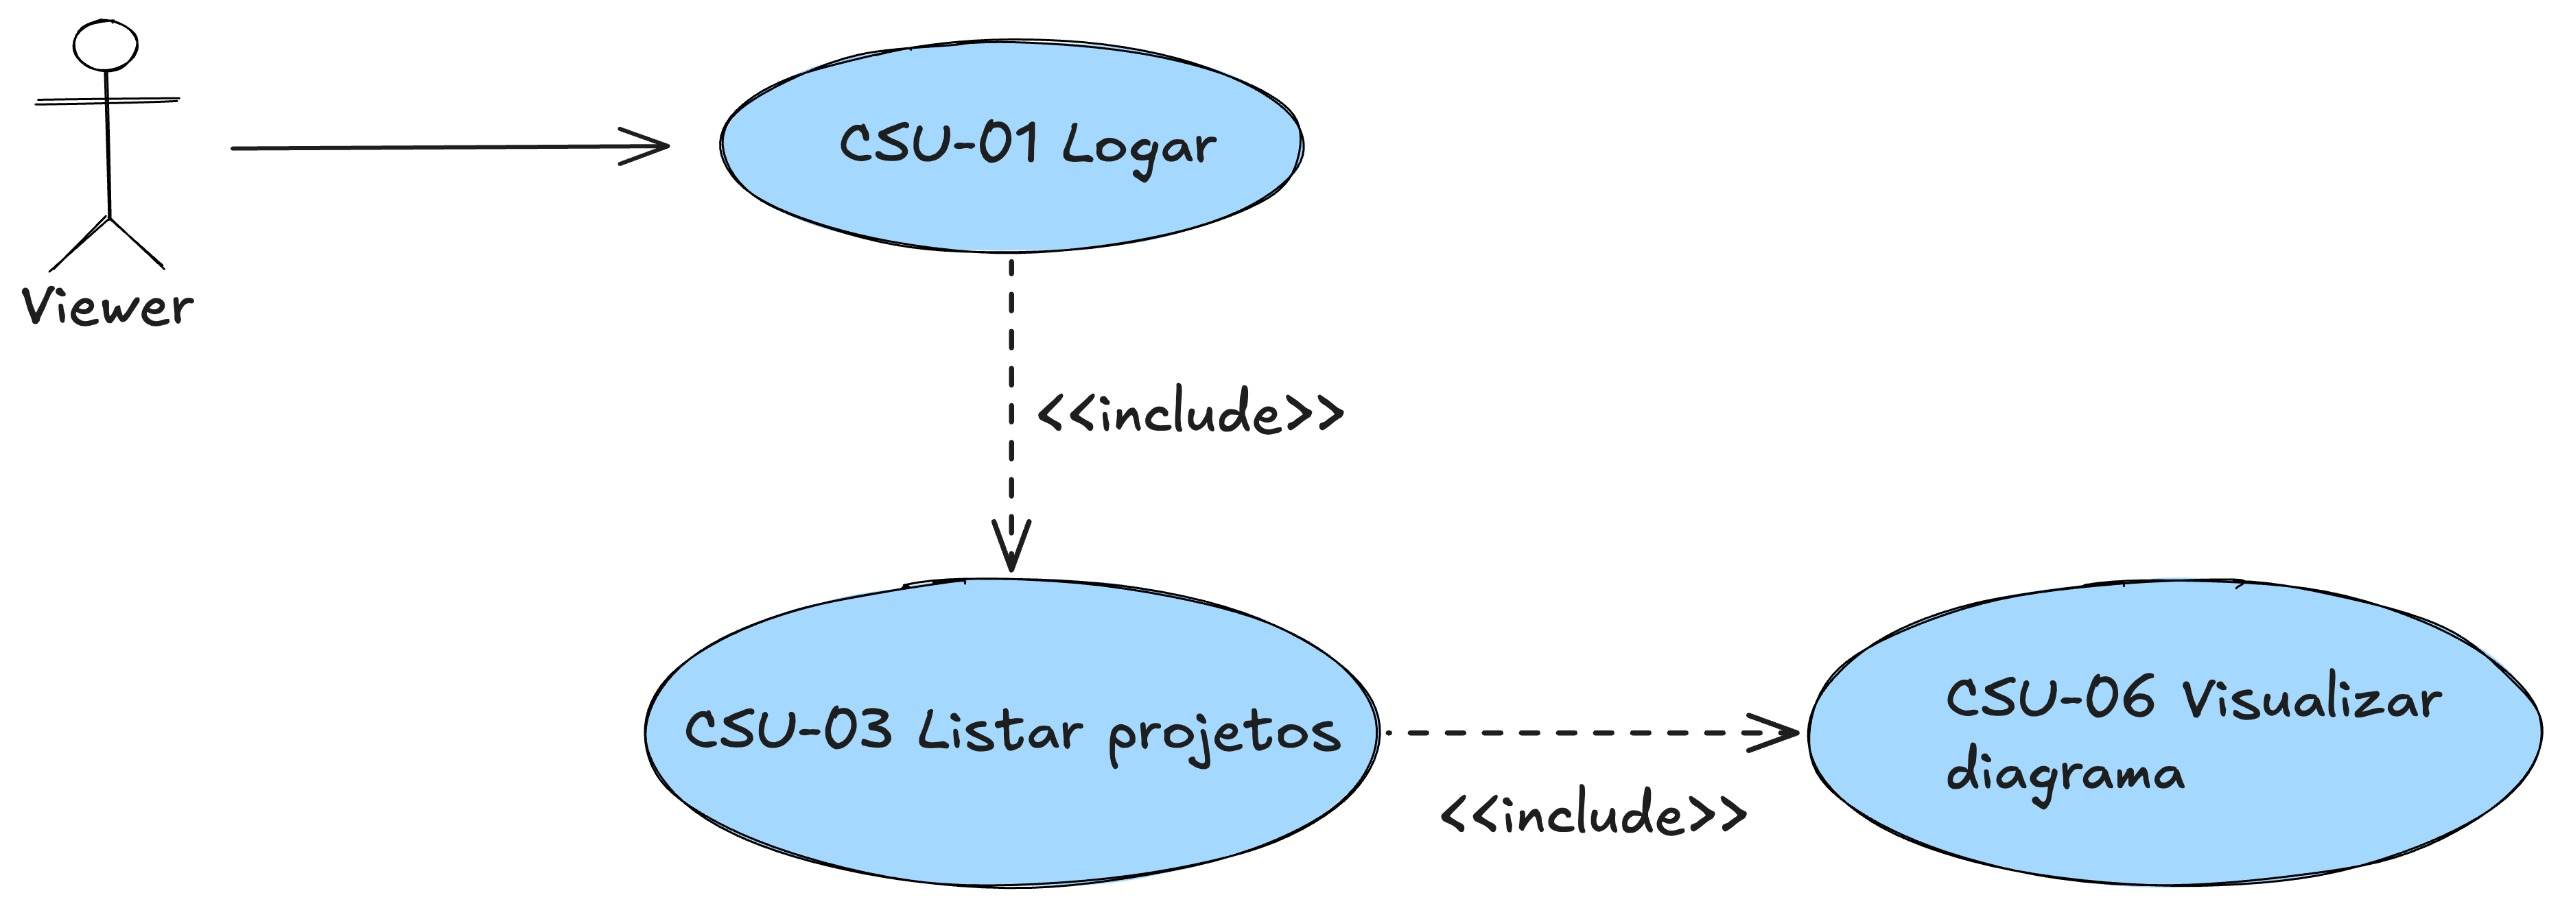
\includegraphics[scale=0.15]{figuras/viewer.jpeg}
    \caption{Diagrama de caso de uso do ator Viewer}
    \begin{center}
        {\small Fonte: Elaborado pelo autor}
    \end{center}
    \label{fig:caso-de-uso-viewer}
\end{figure}

O ator \textit{Editor}, apresentado na Figura~\ref{fig:caso-de-uso-editor}, herda as capacidades do \textit{Viewer} e adiciona a permissão de editar diagramas. Por meio dessa funcionalidade, o \textit{Editor} pode adicionar, editar e remover tabelas, gerenciar os atributos de cada tabela, criar e excluir relacionamentos entre entidades, reposicionar elementos na área de desenho, além de exportar e importar scripts SQL.

\begin{figure}[H]
    \centering
    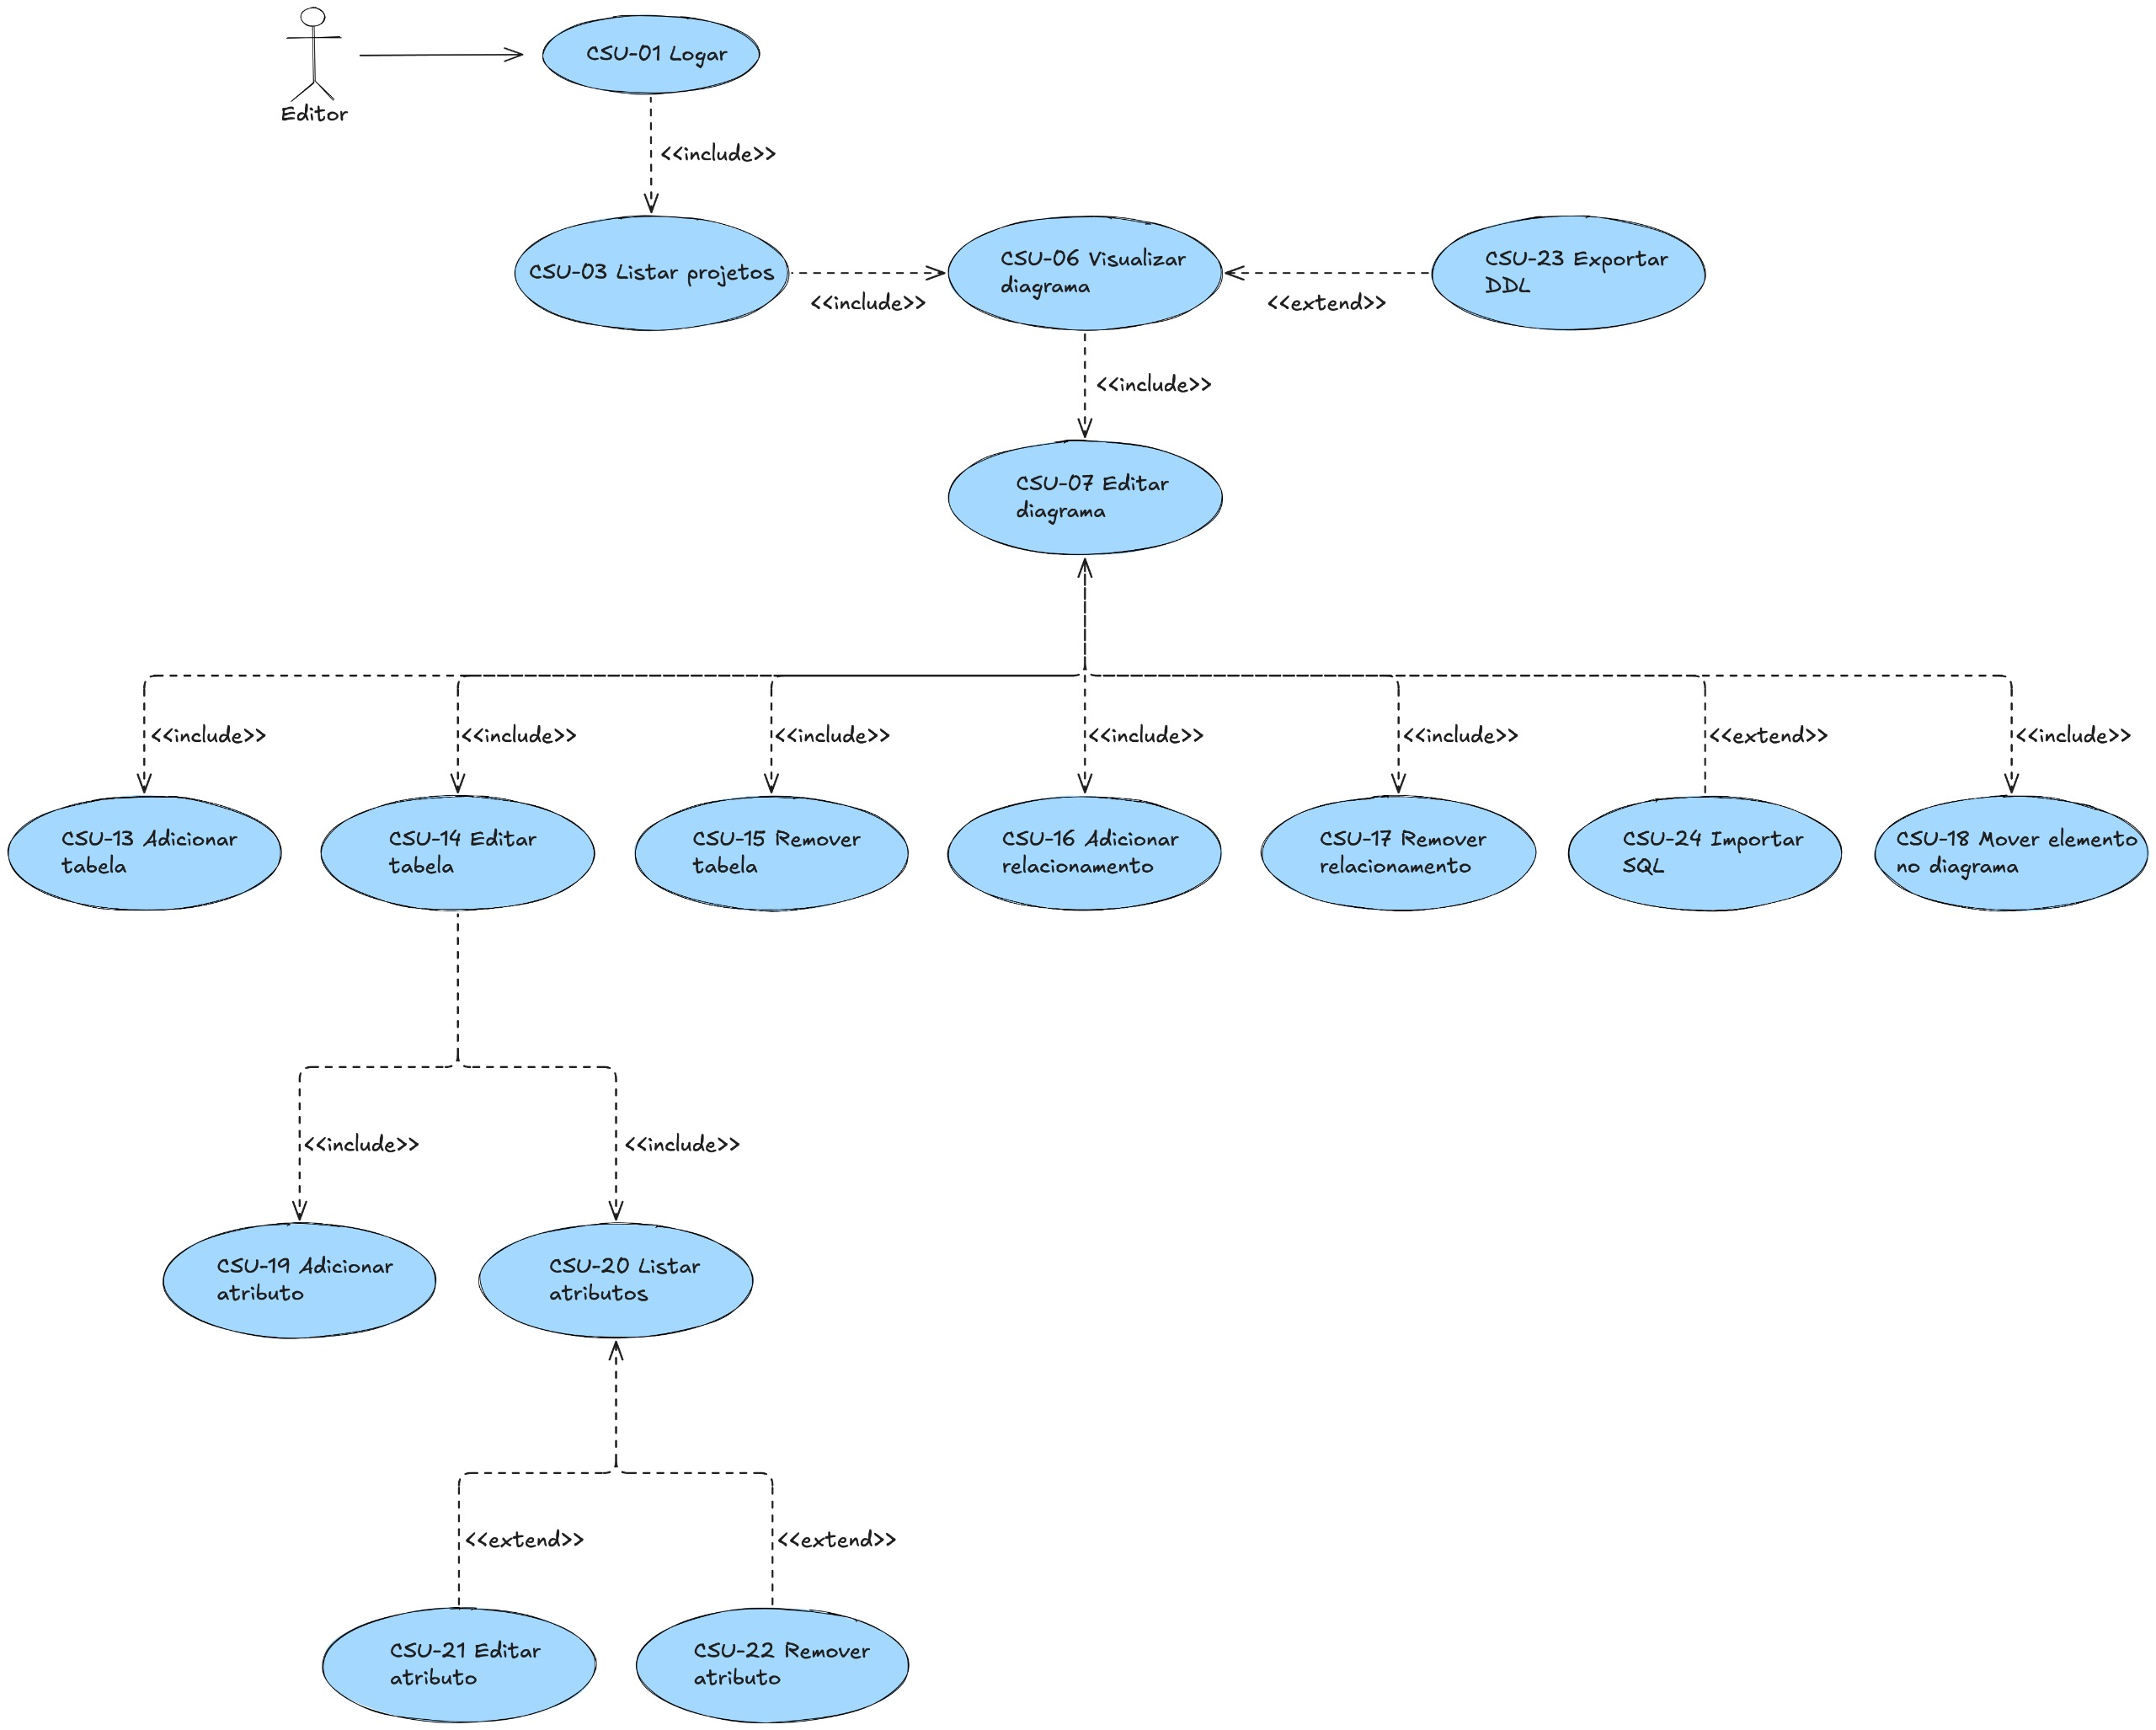
\includegraphics[scale=0.15]{figuras/editor.jpeg}
    \caption{Diagrama de caso de uso do ator Editor}
    \begin{center}
        {\small Fonte: Elaborado pelo autor}
    \end{center}
    \label{fig:caso-de-uso-editor}
\end{figure}

O ator \textit{Owner}, apresentado na Figura~\ref{fig:caso-de-uso-owner}, possui o conjunto mais amplo de permissões. Além de todas as capacidades do \textit{Editor}, o \textit{Owner} é o responsável pelo ciclo de vida dos projetos: pode criá-los, editá-los e removê-los. Também gerencia o time de colaboradores, podendo adicionar membros, listar os membros existentes, alterar seus papéis de acesso e removê-los do projeto.

\begin{figure}[H]
    \centering
    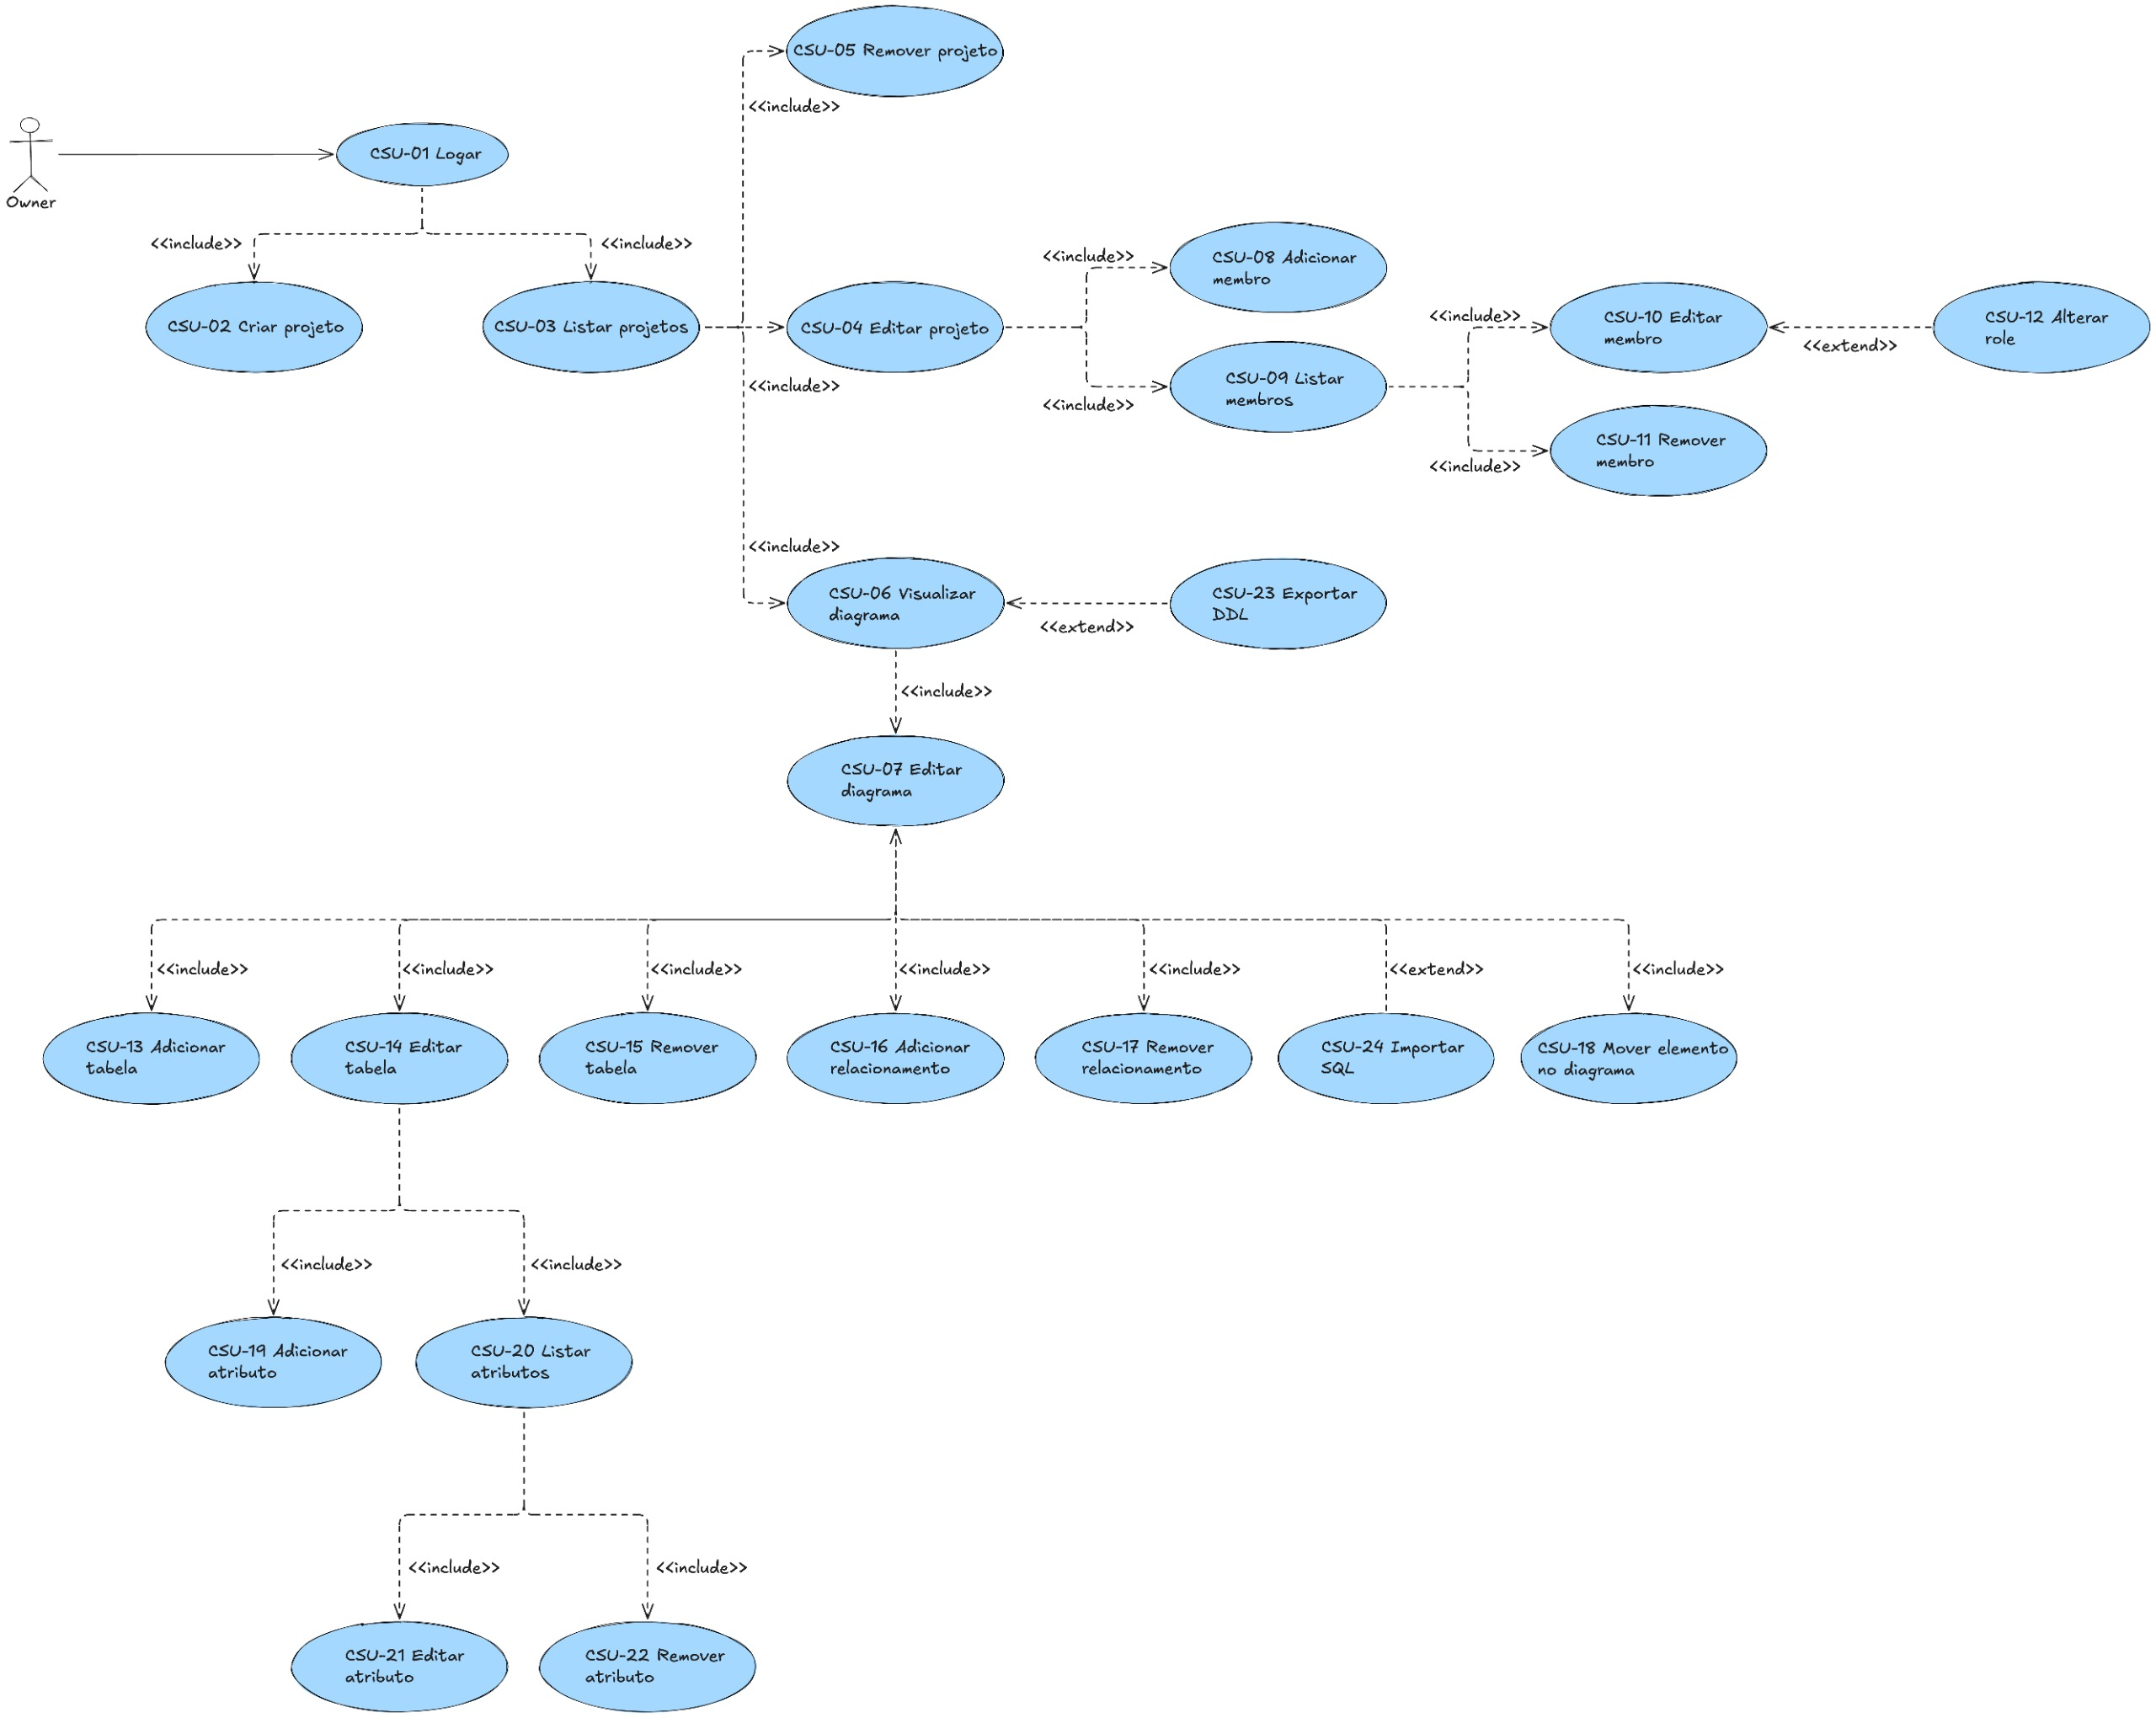
\includegraphics[scale=0.15]{figuras/owner.jpeg}
    \caption{Diagrama de caso de uso do ator Owner}
    \begin{center}
        {\small Fonte: Elaborado pelo autor}
    \end{center}
    \label{fig:caso-de-uso-owner}
\end{figure}

\section{Modelos de Dados}

As figuras \ref{fig:modelo-conceitual}, \ref{fig:modelo-logico} e \ref{fig:modelo-nosql} apresentam, respectivamente, os artefatos de modelagem de dados produzidos no projeto: o modelo conceitual e o modelo lógico do banco de dados relacional, e o esquema não-relacional com MongoDB.

O modelo conceitual define as entidades e relacionamentos de alto nível, representando a estrutura geral dos dados.

\begin{figure}[H]
    \centering
    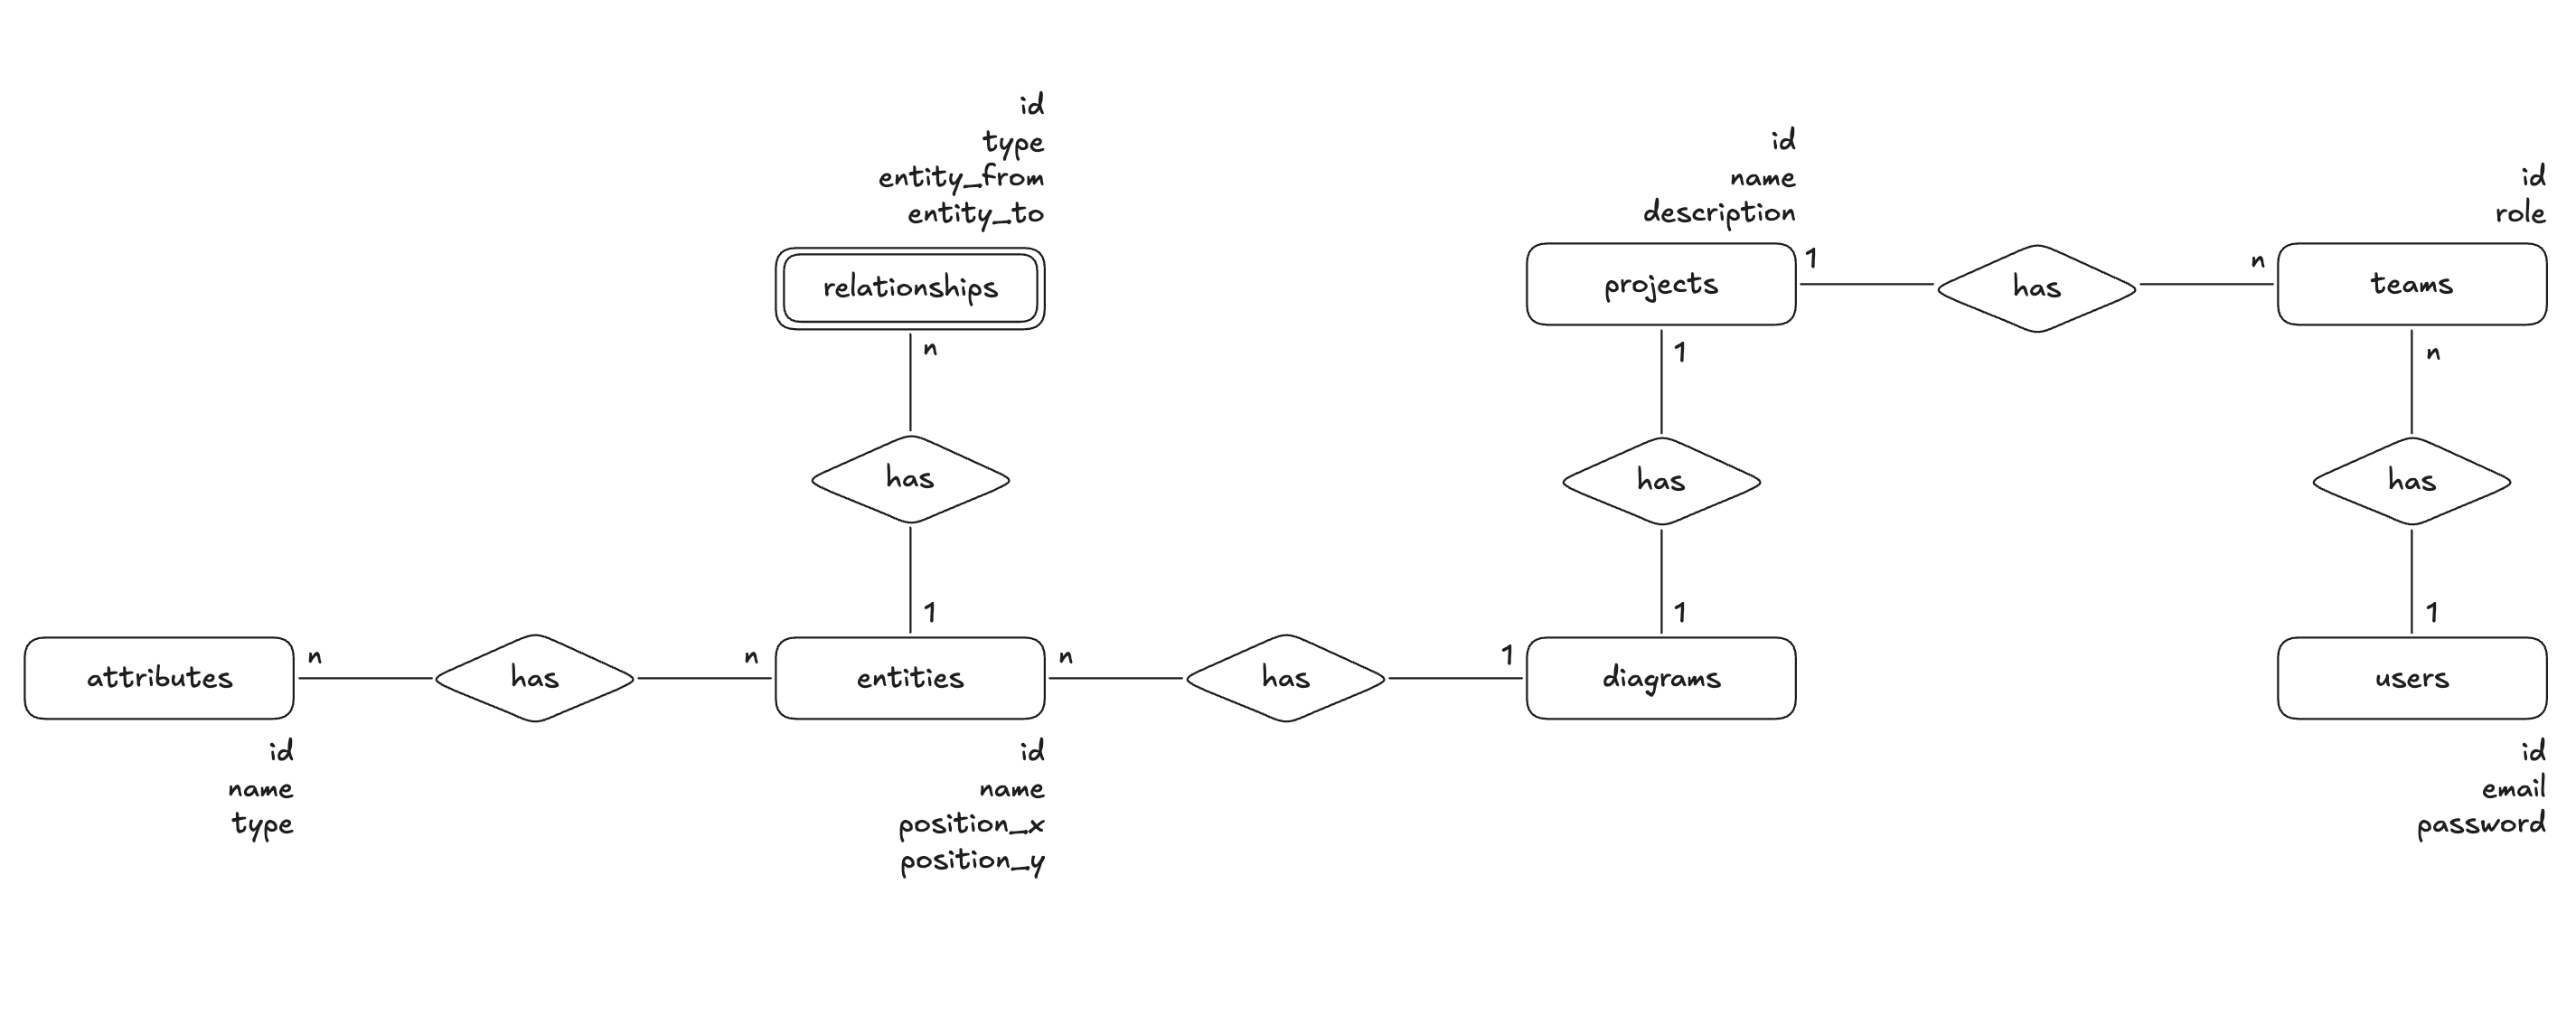
\includegraphics[width=15cm]{figuras/erd-conceptual-model.png}
    \caption{Modelo conceitual do banco de dados}
    \begin{center}
        {\small Fonte: Elaborado pelo autor}
    \end{center}
    \label{fig:modelo-conceitual}
\end{figure}

O modelo lógico detalha a estrutura das tabelas e seus atributos, considerando as características do sistema de gerenciamento de banco de dados utilizado.

\begin{figure}[H]
    \centering
    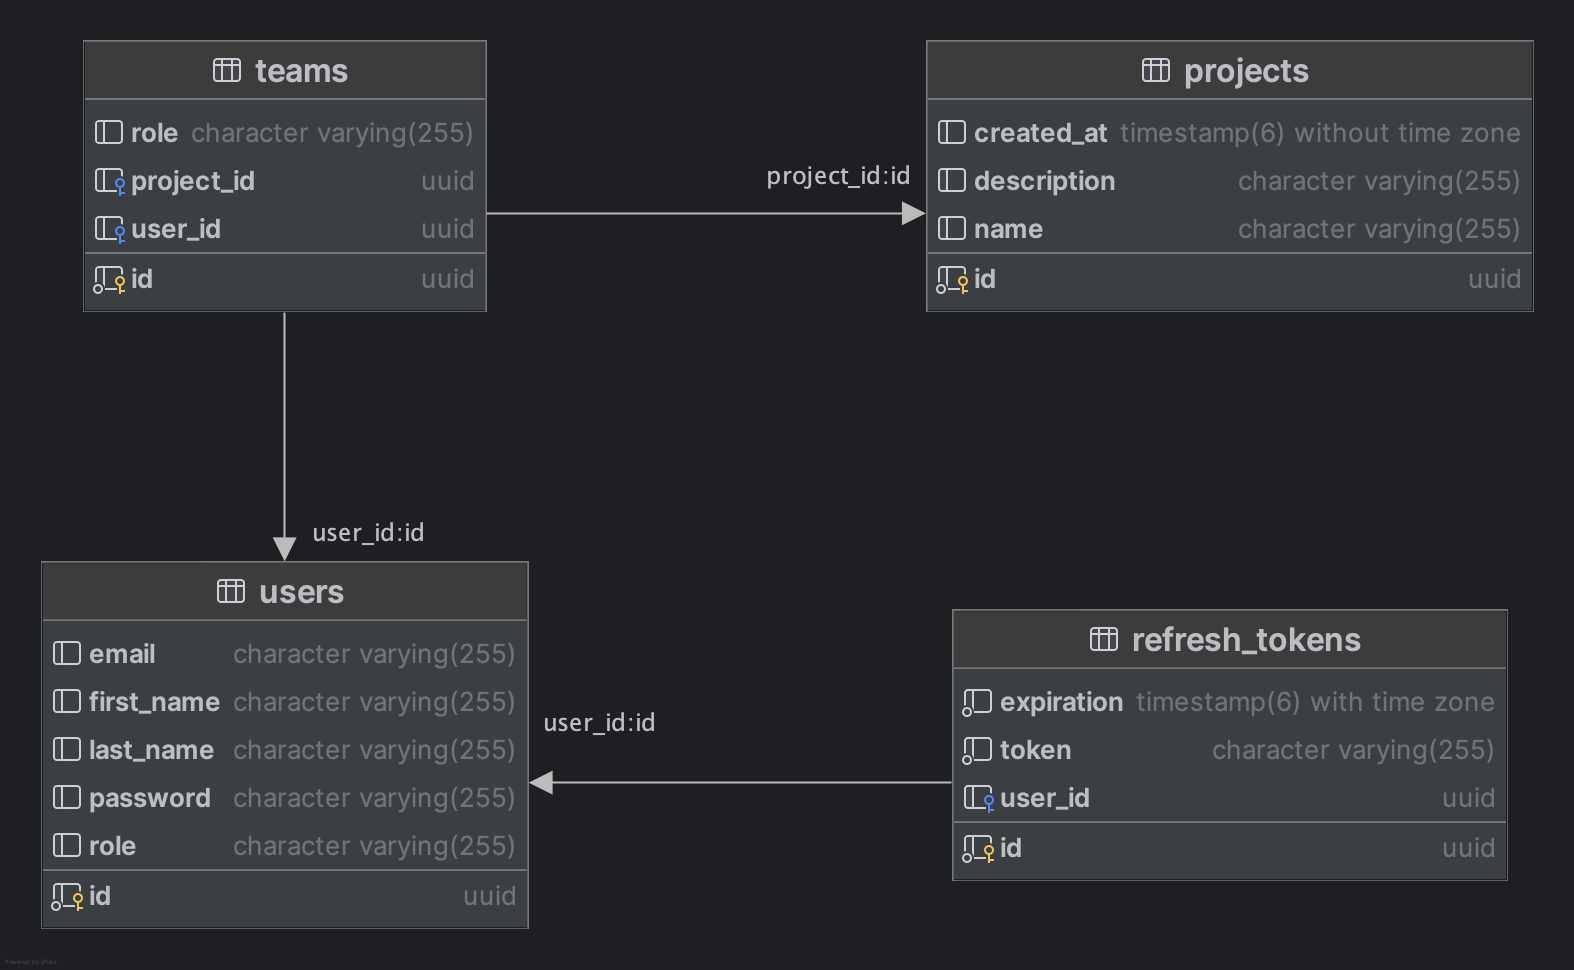
\includegraphics[width=15cm]{figuras/erd-diagram.png}
    \caption{Modelo lógico do banco de dados}
    \begin{center}
        {\small Fonte: Elaborado pelo autor}
    \end{center}
    \label{fig:modelo-logico}
\end{figure}

O esquema documental projetado para o MongoDB contempla as coleções, os campos e os tipos de dados.

\begin{figure}[H]
    \centering
    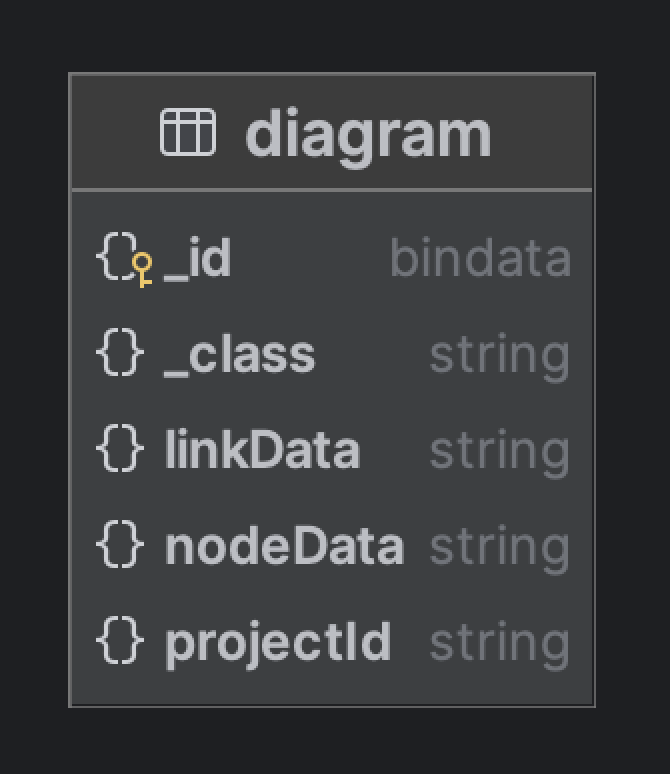
\includegraphics[width=7cm]{figuras/erd-mongodb.png}
    \caption{Esquema do banco de dados não-relacional}
    \begin{center}
        {\small Fonte: Elaborado pelo autor}
    \end{center}
    \label{fig:modelo-nosql}
\end{figure}

Os campos \textit{linkData} e \textit{nodeData} possuem, na devida ordem, os seguintes formatos:

\begin{quadro}[H]
    \begin{lstlisting}
    {
        "from": string,
        "to": string,
        "text": string,
        "toText": interger,
        "fromColumn": string      
    }
    \end{lstlisting}
    \caption{Estrutura de dados do campo \textit{linkData}}
    \begin{center}
        {\small Fonte: Elaborado pelo autor}
    \end{center}
    \label{lst:link-data}
\end{quadro}

\begin{quadro}[H]
    \begin{lstlisting}
    {
        "id": string,
        "key": string,
        "items": [
            {
            "name": string,
            "type": string,
            "pk": boolean,
            "fk": boolean,
            "unique": boolean,
            "notNull": boolean,
            "autoIncrement": boolean,
            "defaultValue": string
            }
        ],
        "location": {
            "x": string,
            "y": string
        }
    }
    \end{lstlisting}
    \caption{Estrutura de dados do campo \textit{nodeData}}
    \begin{center}
        {\small Fonte: Elaborado pelo autor}
    \end{center}
    \label{lst:node-data}
\end{quadro}

\section{Arquitetura do Protótipo}

O protótipo foi construído segundo a arquitetura cliente-servidor, composta por dois módulos independentes: o \textit{back-end}, implementado com Spring Boot, e o \textit{front-end}, desenvolvido com Angular. A Figura~\ref{fig:arquitetura} apresenta uma visão geral dos componentes do sistema e dos canais de comunicação entre eles.

\begin{figure}[H]
    \centering
    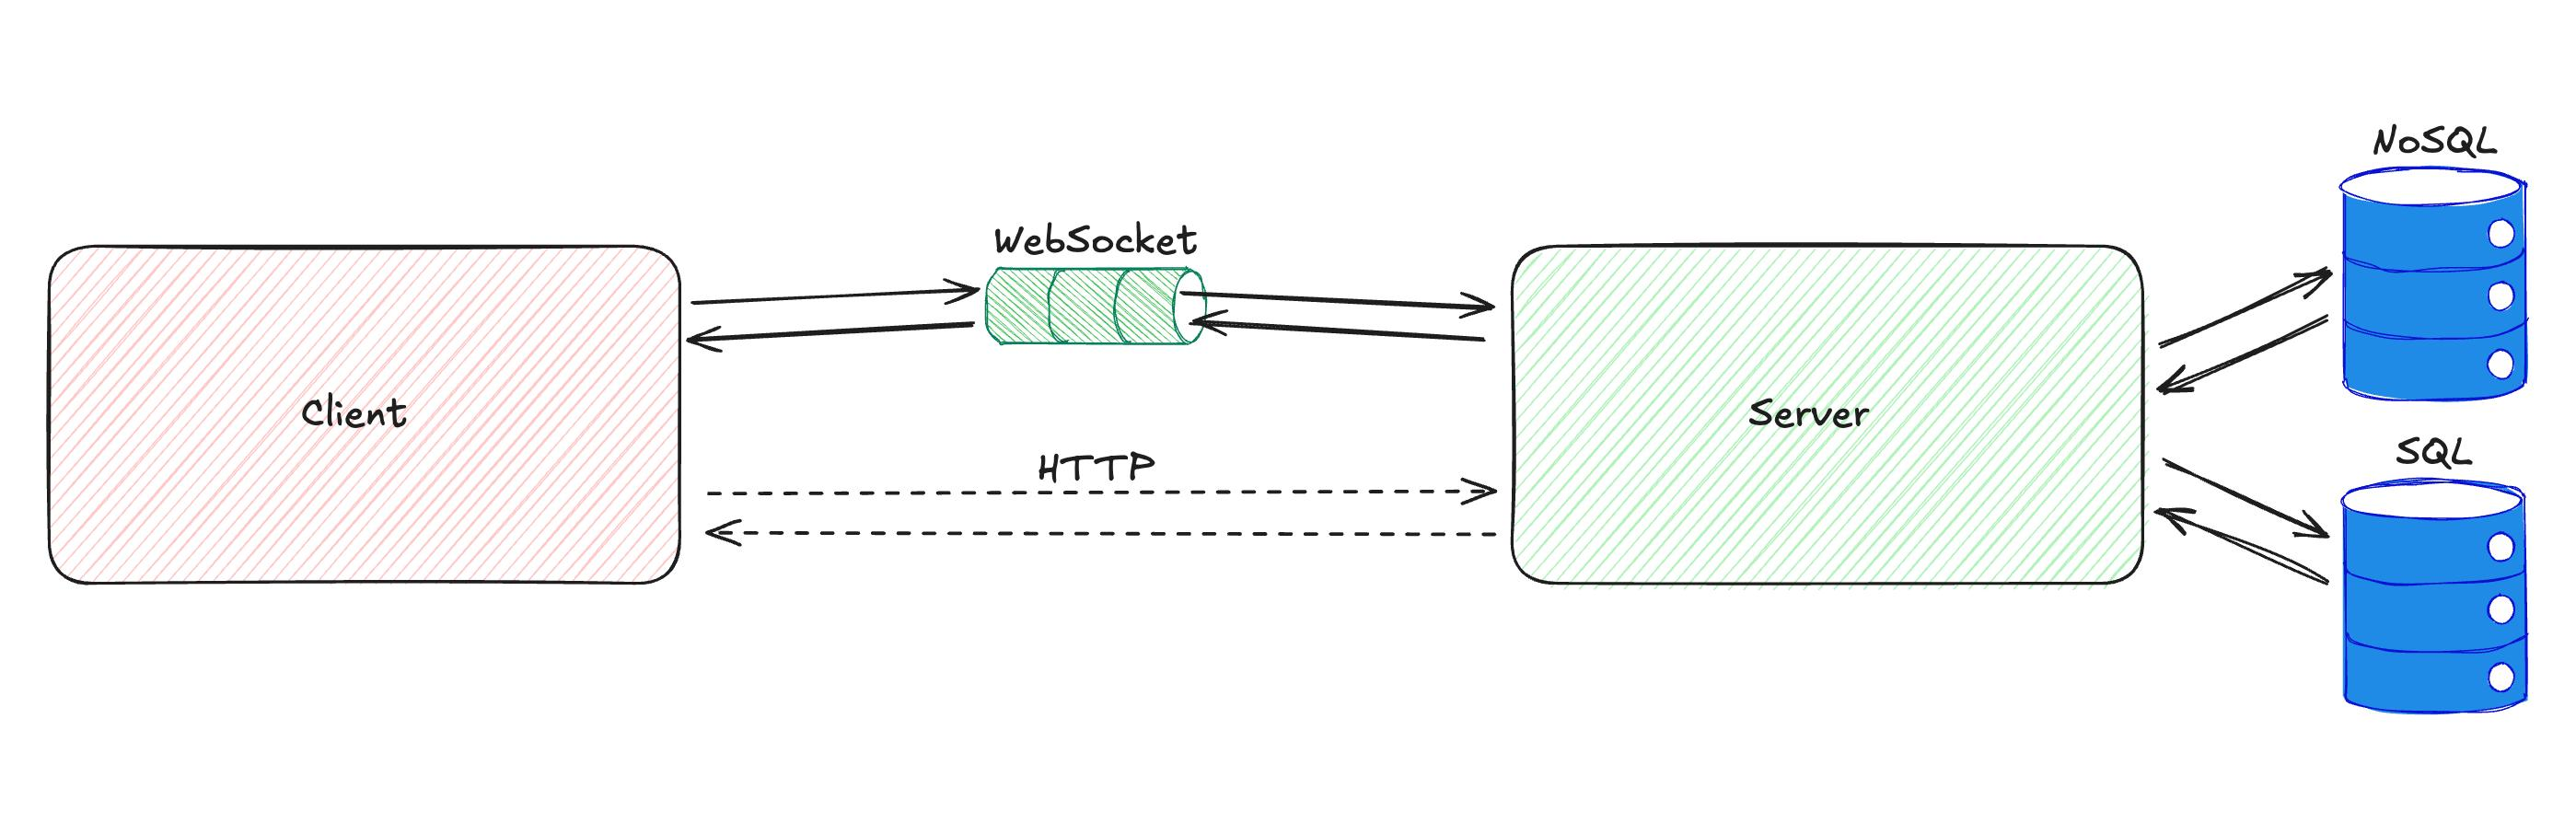
\includegraphics[width=15cm]{figuras/desenho-da-arquitetura.jpeg}
    \caption{Arquitetura do protótipo}
    \begin{center}
        {\small Fonte: Elaborado pelo autor}
    \end{center}
    \label{fig:arquitetura}
\end{figure}

A comunicação entre os módulos ocorre por dois canais distintos: requisições HTTP para as operações de persistência e autenticação, e uma conexão persistente via WebSocket para a sincronização colaborativa em tempo real.

O \textit{back-end} foi organizado em camadas seguindo o padrão MVC, separando as responsabilidades de controle, regras de negócio e acesso a dados. A segurança da API é gerenciada por meio de \textit{tokens} JWT armazenados em \textit{cookies} no navegador do cliente, protegendo os recursos contra acesso não autorizado. A comunicação em tempo real é viabilizada por um servidor WebSocket dedicado, responsável por receber as ações dos colaboradores e propagá-las a todos os usuários conectados ao mesmo projeto.

O \textit{front-end} é estruturado como uma SPA, com responsabilidades distribuídas entre componentes de interface, serviços de dados e interceptadores de requisição. O componente central do editor integra a biblioteca GoJS para a renderização e manipulação interativa do diagrama no \textit{canvas}, enquanto serviços dedicados encapsulam a comunicação em tempo real e as operações de importação e exportação SQL.

\section{Funcionalidades Implementadas}

As subseções a seguir descrevem as funcionalidades que compõem o protótipo desenvolvido.

\subsection{Autenticação e Autorização}

O protótipo implementa um fluxo de autenticação com credenciais de acesso. Após a autenticação bem-sucedida, o servidor emite dois \textit{tokens} de segurança: um de curta duração para as requisições e outro de renovação, ambos armazenados de forma segura no navegador do cliente. As rotas da aplicação são protegidas tanto no lado do cliente quanto no servidor, garantindo que apenas usuários autenticados acessem os recursos. Quando o \textit{token} de acesso expira, a renovação ocorre de forma automática e transparente ao usuário, sem necessidade de novo \textit{login}.

A Figura~\ref{fig:arquitetura-autenticacao} ilustra a arquitetura de autenticação e autorização implementada no \textit{back-end}. Toda requisição originada pelo cliente passa pelo filtro JWT, que valida o \textit{token} presente no \textit{cookie}; caso inválido, a requisição é rejeitada com o código 401 (\textit{Unauthorized}). Requisições válidas avançam para duas camadas de autorização em série: a primeira verifica permissões com base na URL acessada e a segunda aplica restrições mais granulares ao nível do método, controlando o acesso de acordo com o perfil do usuário autenticado. O descumprimento de qualquer uma dessas camadas resulta em resposta 403 (\textit{Forbidden}); somente após a aprovação em ambas a requisição alcança os controladores da aplicação.

\begin{figure}[H]
    \centering
    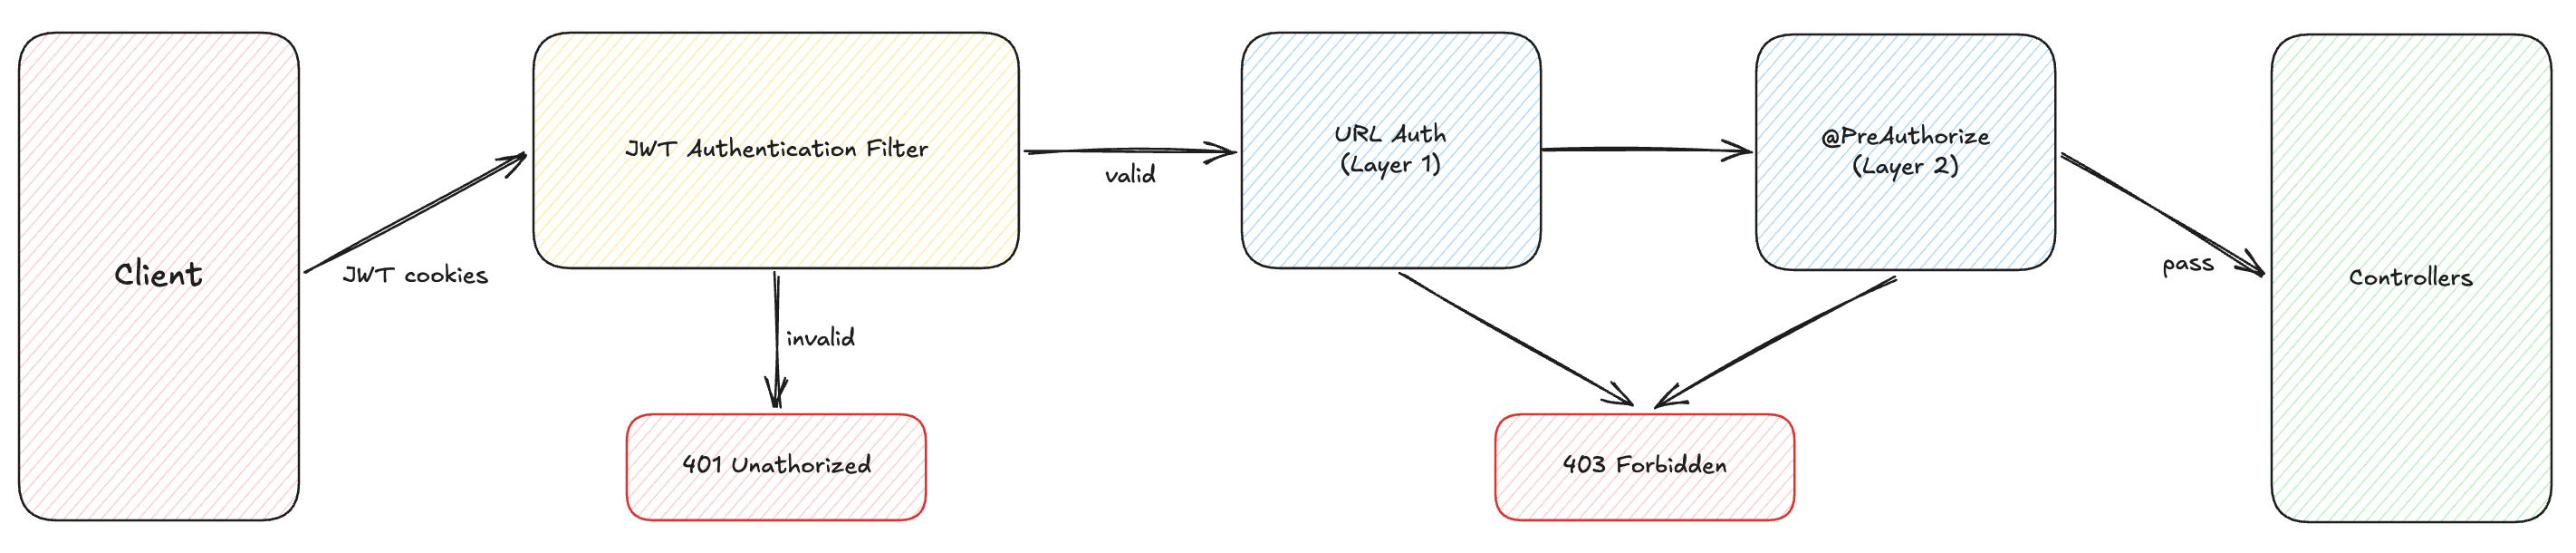
\includegraphics[width=\textwidth]{figuras/desenho-da-arquitetura-de-autenticacao-e-autorizacao.jpeg}
    \caption{Arquitetura de autenticação e autorização do \textit{back-end}}
    \begin{center}
        {\small Fonte: Elaborado pelo autor}
    \end{center}
    \label{fig:arquitetura-autenticacao}
\end{figure}

\subsection{Gerenciamento de Projetos e Times}

O sistema permite ao usuário criar e gerenciar projetos de modelagem. Cada projeto possui um time de colaboradores, para o qual o criador pode convidar outros usuários cadastrados na plataforma. A gestão de projetos e times é realizada por meio de uma interface de \textit{dashboard}, com operações de criação, leitura, atualização e exclusão comunicadas ao servidor e persistidas no banco de dados.

\subsection{Editor de Diagramas ER}

O editor de diagramas constitui o componente central do protótipo. Construído com a biblioteca GoJS, o \textit{canvas} permite adicionar e remover entidades (tabelas), gerenciar seus atributos com configuração de tipo de dado, chave primária, chave estrangeira, unicidade, restrição não nulo, auto-incremento e valor padrão, criar e excluir relacionamentos entre entidades com definição de cardinalidade, além de reposicionar livremente os elementos na área de desenho. O estado completo do diagrama (entidades, atributos, relacionamentos e posicionamentos) é persistido na base de dados ao final de cada sequência de ações.

\subsection{Colaboração em Tempo Real}

A funcionalidade de colaboração permite que múltiplos usuários de um mesmo time trabalhem simultaneamente no mesmo diagrama. Ao abrir um projeto, o cliente estabelece automaticamente uma conexão persistente com o servidor para receber atualizações em tempo real. Quando um usuário seleciona uma entidade para edição, uma notificação de bloqueio é imediatamente propagada a todos os demais colaboradores conectados. Enquanto o bloqueio está ativo, a entidade correspondente fica indisponível para edição pelos outros usuários, prevenindo conflitos de concorrência. O bloqueio é liberado automaticamente pelo servidor após um intervalo de tempo predefinido, caso o usuário não o libere explicitamente.

\subsection{Importação e Exportação de Diagramas}

O protótipo suporta a interoperabilidade com outros ambientes por meio de operações SQL no dialeto MySQL. A exportação converte o modelo do diagrama em instruções SQL de criação de tabelas, enquanto a importação analisa um \textit{script} SQL fornecido pelo usuário para reconstruir o diagrama correspondente no \textit{canvas}. Ambas as operações são processadas pelo \textit{back-end} e o resultado é retornado ao usuário pela interface da aplicação.

\section{\textit{Interface} do Usuário}

Esta seção apresenta as telas que compõem a \textit{interface} do protótipo, organizadas pelo fluxo de uso da aplicação.

% ----------------------------------------------------------
\subsection{Autenticação}
% ----------------------------------------------------------

A Figura~\ref{fig:tela-login} apresenta a tela de entrada da aplicação. O usuário informa seu \textit{e-mail} e senha para autenticar-se, com a opção de manter a sessão ativa. O cadastro de novos usuários não está disponível pela interface gráfica, sendo realizado exclusivamente por meio da API do \textit{back-end}. O Quadro~\ref{lst:curl-cadastro} apresenta o comando utilizado para esse cadastro.

\begin{figure}[H]
    \centering
    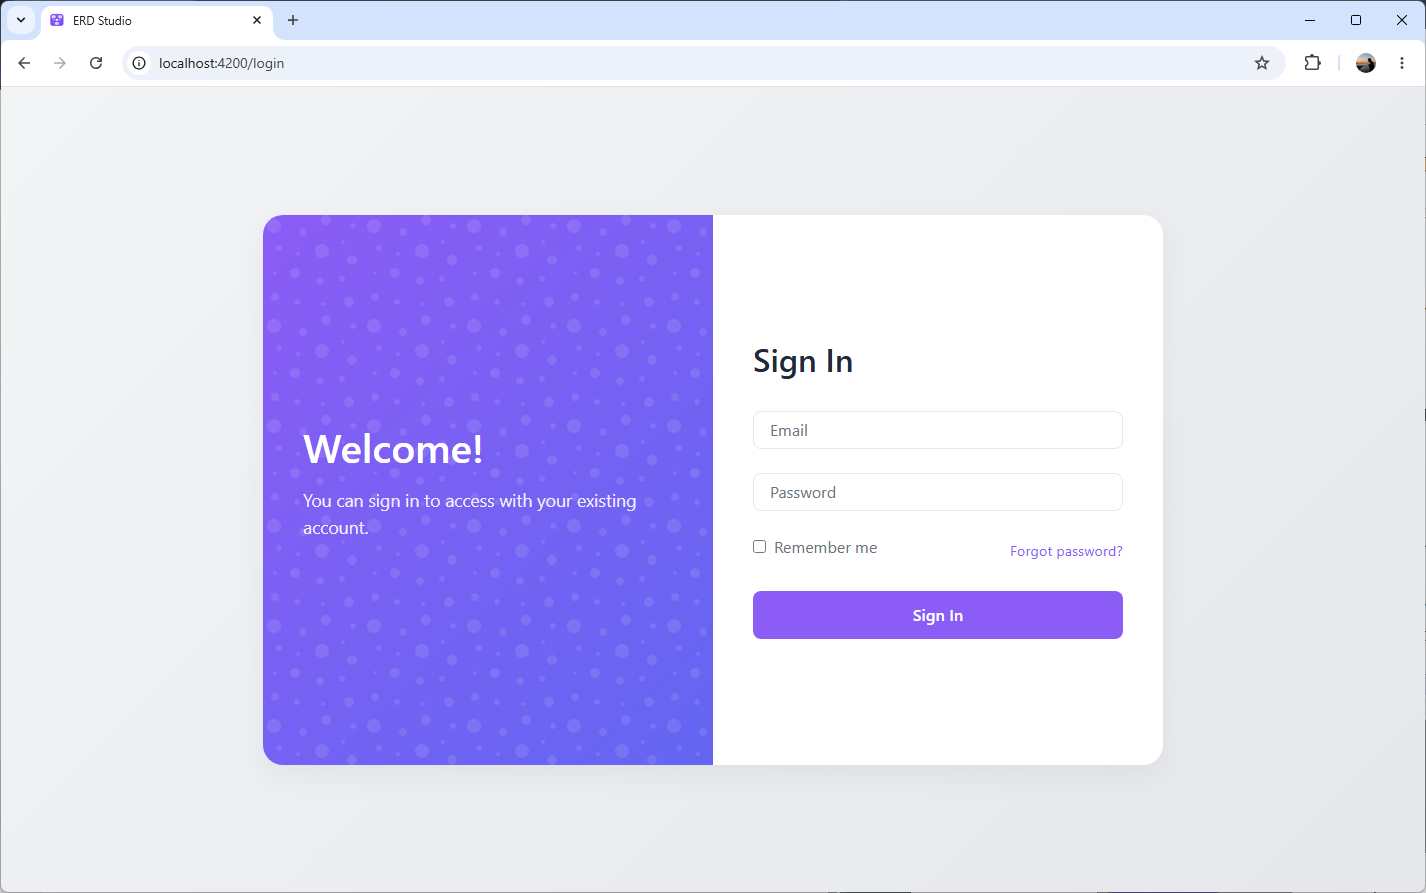
\includegraphics[width=15cm]{figuras/interface/tela-de-login.png}
    \caption{Tela de \textit{login}}
    \begin{center}
        {\small Fonte: Elaborado pelo autor}
    \end{center}
    \label{fig:tela-login}
\end{figure}

\begin{quadro}[H]
    \begin{lstlisting}
curl -X POST http://localhost:8080/api/user \
    -H "Content-Type: application/json" \
    -d '{
      "firstName": "Test",
      "lastName": "Name",
      "email": "test.name@email.com",
      "password": "yourPassword123!",
      "role": "USER"
    }'
    \end{lstlisting}
    \caption{Comando para cadastro de usuário via API}
    \begin{center}
        {\small Fonte: Elaborado pelo autor}
    \end{center}
    \label{lst:curl-cadastro}
\end{quadro}

% ----------------------------------------------------------
\subsection{Gerenciamento de Projetos e Times}
% ----------------------------------------------------------

Após o \textit{login}, o usuário é direcionado à tela principal da aplicação, apresentada na Figura~\ref{fig:tela-principal}. O menu lateral lista os projetos dos quais o usuário faz parte e disponibiliza o botão para criação de um novo projeto. Na parte inferior do menu, são exibidas as informações do usuário autenticado e a opção de encerrar a sessão.

\begin{figure}[H]
    \centering
    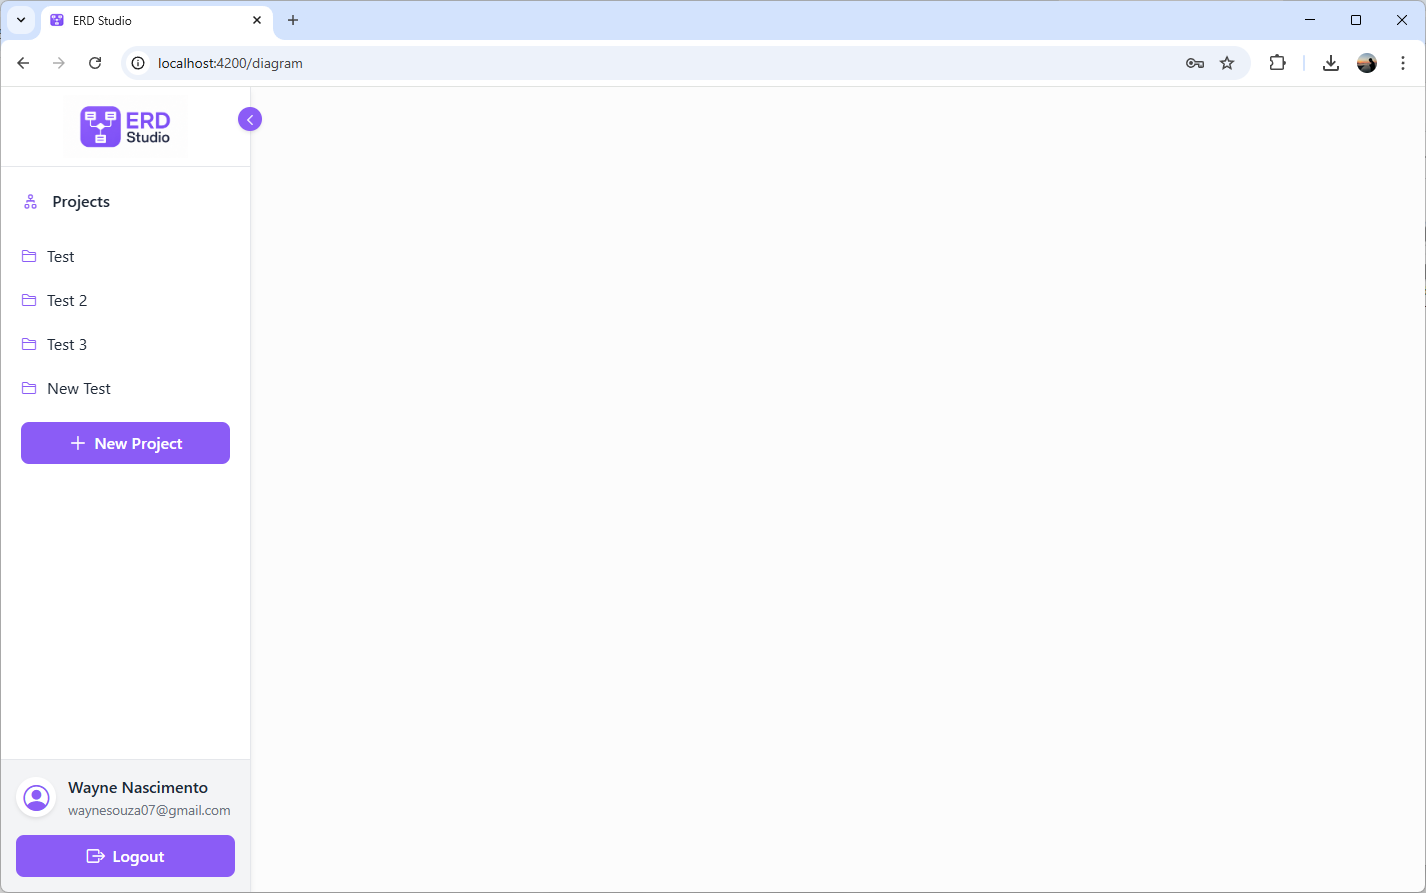
\includegraphics[width=15cm]{figuras/interface/tela-principal.png}
    \caption{Tela principal com listagem de projetos}
    \begin{center}
        {\small Fonte: Elaborado pelo autor}
    \end{center}
    \label{fig:tela-principal}
\end{figure}

Ao acionar o botão de criação, é exibido o \textit{modal} apresentado na Figura~\ref{fig:criacao-projeto}. O usuário informa o nome e a descrição do projeto e confirma a operação. O projeto criado passa a aparecer imediatamente no menu lateral.

\begin{figure}[H]
    \centering
    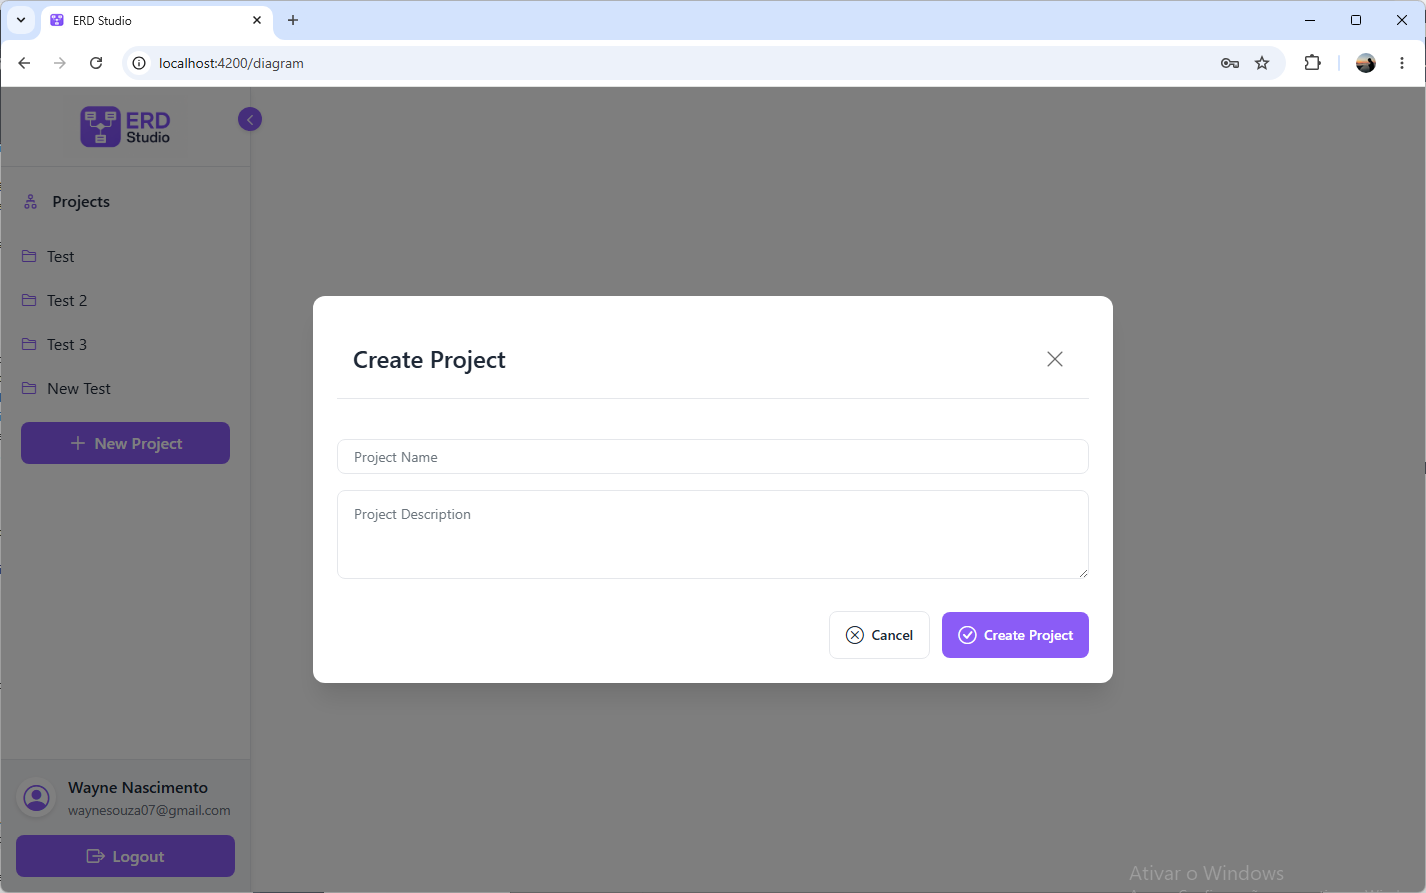
\includegraphics[width=15cm]{figuras/interface/modal-de-criacao-de-projeto.png}
    \caption{\textit{Modal} de criação de projeto}
    \begin{center}
        {\small Fonte: Elaborado pelo autor}
    \end{center}
    \label{fig:criacao-projeto}
\end{figure}

A Figura~\ref{fig:edicao-projeto} ilustra o \textit{modal} de edição de projeto, que reúne em uma única tela a edição dos dados do projeto e o gerenciamento do time de colaboradores. A seção \textit{Team Members} lista os membros com seus respectivos papéis de acesso, e o \textit{Owner} pode adicionar ou remover colaboradores e alterar seus papéis. A tela também disponibiliza a opção de excluir o projeto.

\begin{figure}[H]
    \centering
    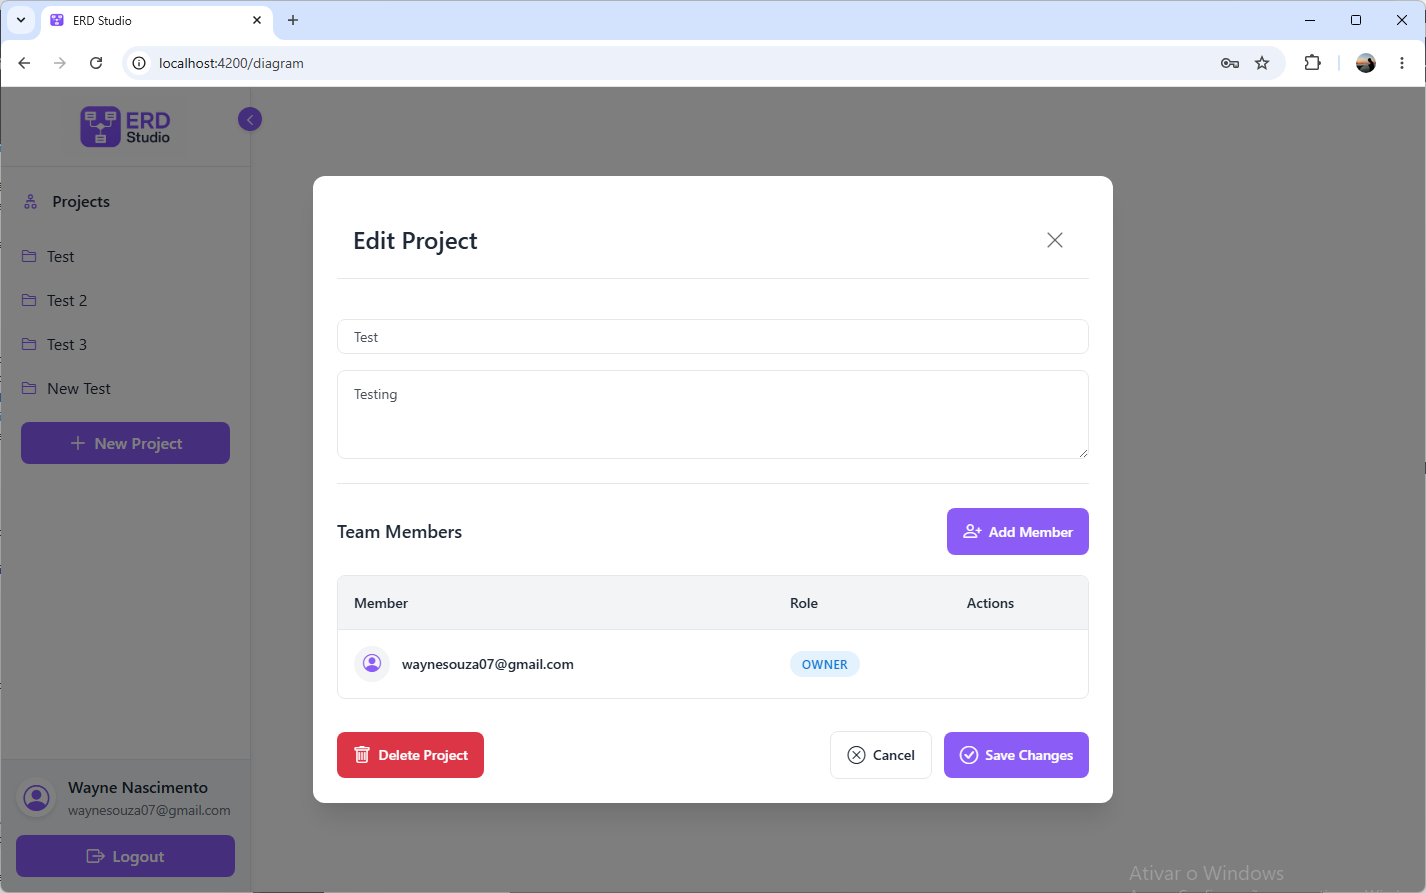
\includegraphics[width=15cm]{figuras/interface/modal-de-edicao-de-projeto.png}
    \caption{\textit{Modal} de edição de projeto e gerenciamento de time}
    \begin{center}
        {\small Fonte: Elaborado pelo autor}
    \end{center}
    \label{fig:edicao-projeto}
\end{figure}

A adição de um novo membro é realizada por meio de um \textit{modal} secundário, apresentado na Figura~\ref{fig:adicionar-membro}. O \textit{Owner} informa o e-mail do colaborador e seleciona o papel de acesso a ser atribuído (\textit{Viewer} ou \textit{Editor}).

\begin{figure}[H]
    \centering
    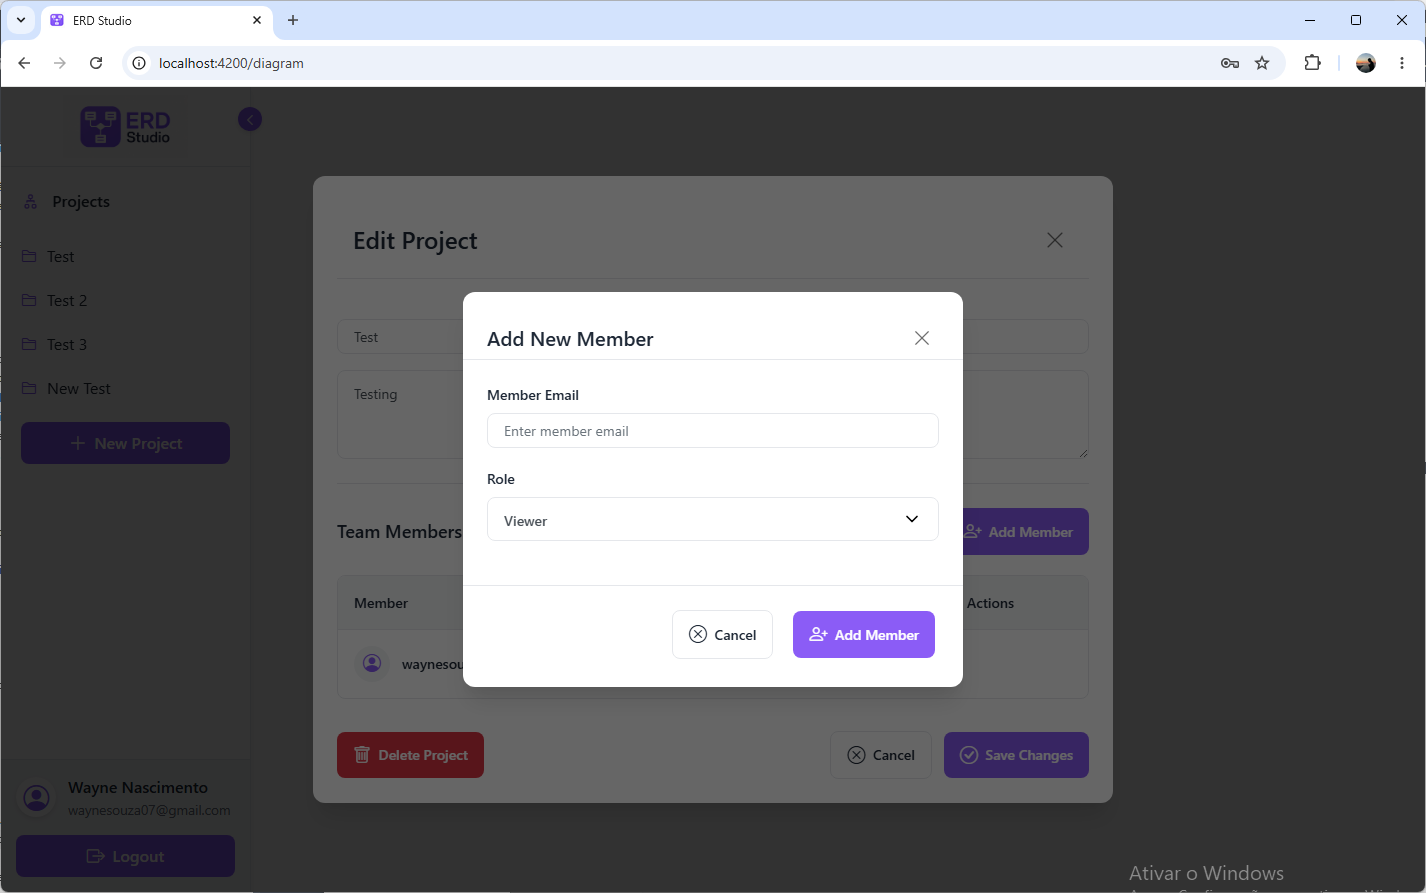
\includegraphics[width=15cm]{figuras/interface/modal-de-adicao-de-membro-no-projeto.png}
    \caption{\textit{Modal} de adição de membro ao projeto}
    \begin{center}
        {\small Fonte: Elaborado pelo autor}
    \end{center}
    \label{fig:adicionar-membro}
\end{figure}

% ----------------------------------------------------------
\subsection{Editor de Diagramas}
% ----------------------------------------------------------

Ao selecionar um projeto no menu lateral, o usuário acessa o editor de diagramas. A Figura~\ref{fig:diagrama-vazio} apresenta o editor com um diagrama composto por três entidades e seus respectivos relacionamentos. A barra de ferramentas lateral disponibiliza as ações de modelagem: adição de entidade, definição do tipo de relacionamento e operações de importação e exportação SQL. No topo da tela, o papel do usuário no projeto é exibido em destaque.

\begin{figure}[H]
    \centering
    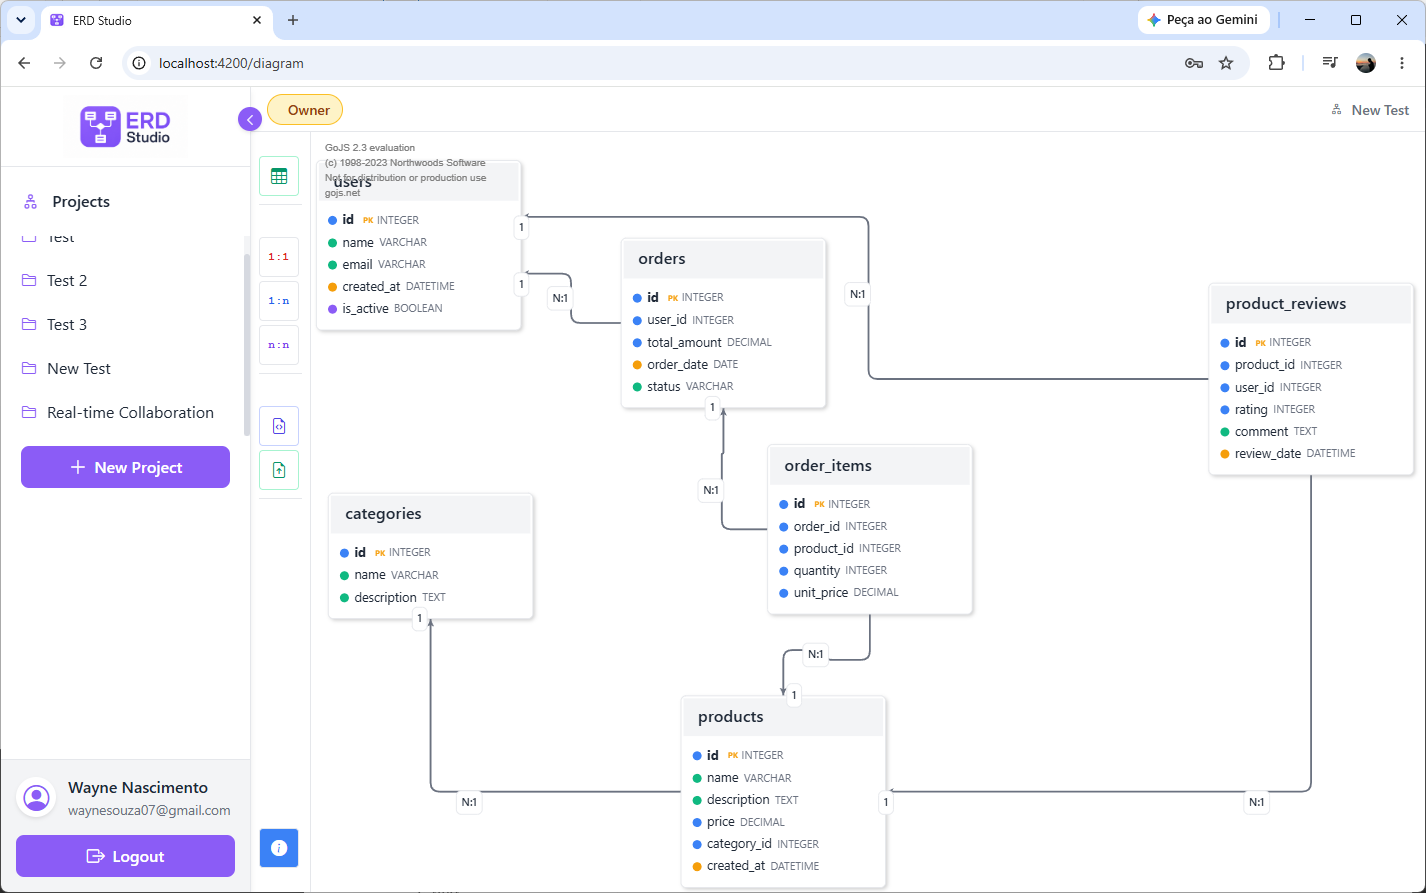
\includegraphics[width=15cm]{figuras/interface/tela-com-diagrama-simples.png}
    \caption{Editor de diagramas com entidades e relacionamentos}
    \begin{center}
        {\small Fonte: Elaborado pelo autor}
    \end{center}
    \label{fig:diagrama-vazio}
\end{figure}

Ao adicionar ou selecionar uma entidade no \textit{canvas}, o \textit{modal} de edição apresentado na Figura~\ref{fig:edicao-entidade} é exibido. O usuário define o nome da entidade e gerencia seus atributos por meio de uma tabela interativa. Para cada atributo, é possível configurar o nome, o tipo de dado e as restrições aplicáveis: chave primária, unicidade, obrigatoriedade, auto-incremento e valor padrão. Novos atributos são adicionados por meio do botão disponível no rodapé do \textit{modal}.

\begin{figure}[H]
    \centering
    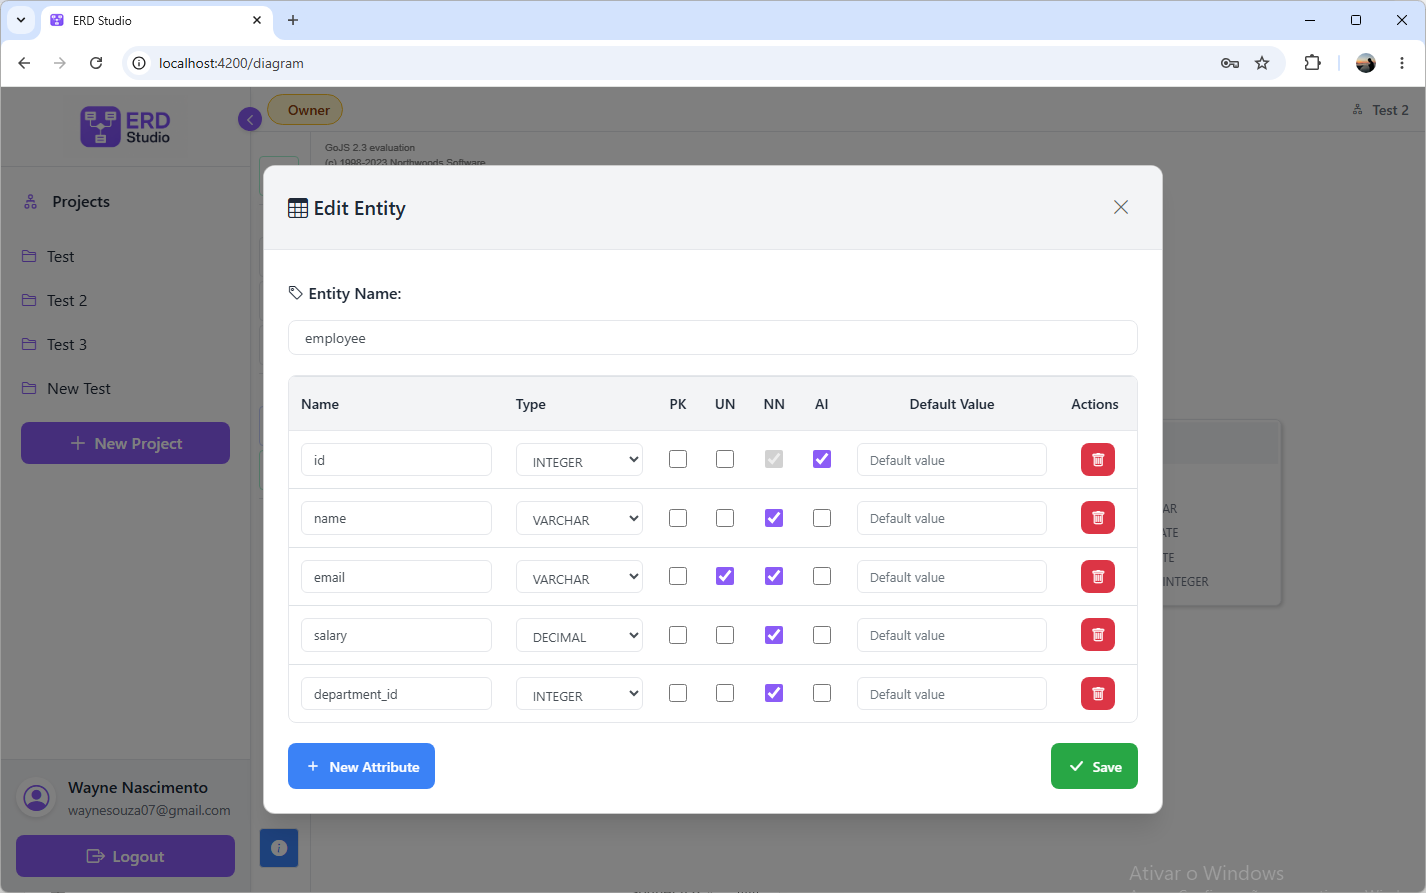
\includegraphics[width=15cm]{figuras/interface/modal-de-edicao-da-tabela.png}
    \caption{\textit{Modal} de edição de entidade}
    \begin{center}
        {\small Fonte: Elaborado pelo autor}
    \end{center}
    \label{fig:edicao-entidade}
\end{figure}

A Figura~\ref{fig:diagrama-com-entidades} exibe o mesmo diagrama com a legenda visível no \textit{canvas}. A legenda descreve o código de cores utilizado para representar os tipos de dados dos atributos e indica os marcadores de chave primária. O diagrama reflete em tempo real as alterações realizadas por qualquer colaborador conectado ao projeto.

\begin{figure}[H]
    \centering
    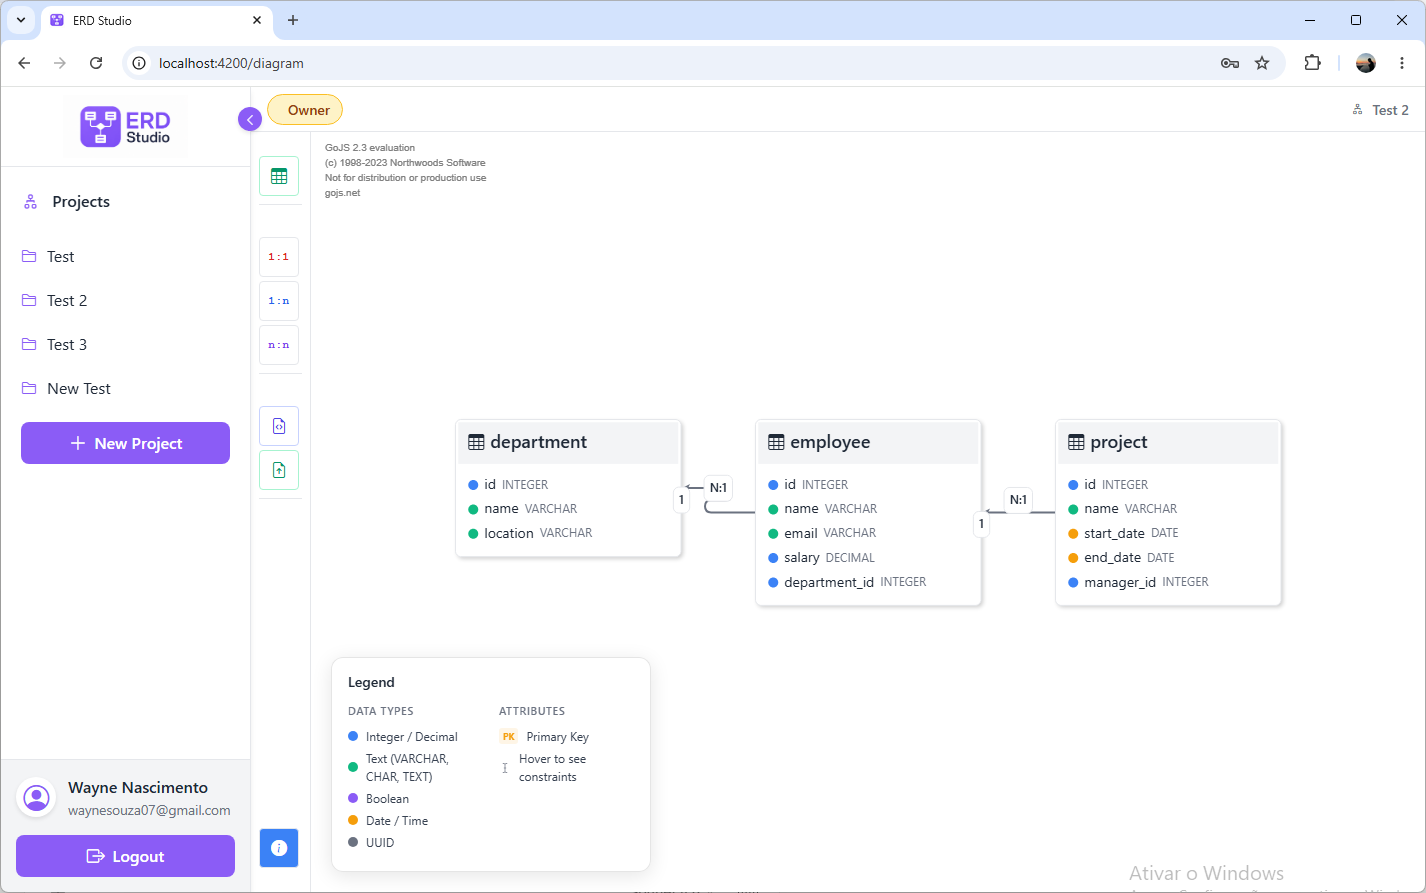
\includegraphics[width=15cm]{figuras/interface/tela-com-diagrama-simples-e-com-legenda.png}
    \caption{Editor de diagramas com legenda de tipos de dados}
    \begin{center}
        {\small Fonte: Elaborado pelo autor}
    \end{center}
    \label{fig:diagrama-com-entidades}
\end{figure}

Quando um usuário acessa um projeto com o papel de \textit{Viewer}, o editor é exibido em modo somente leitura. Conforme ilustra a Figura~\ref{fig:perfil-viewer}, a barra lateral de ferramentas é substituída por um indicador de visualização, impedindo qualquer operação de criação ou edição no diagrama. O papel atribuído ao usuário é exibido no topo da tela.

\begin{figure}[H]
    \centering
    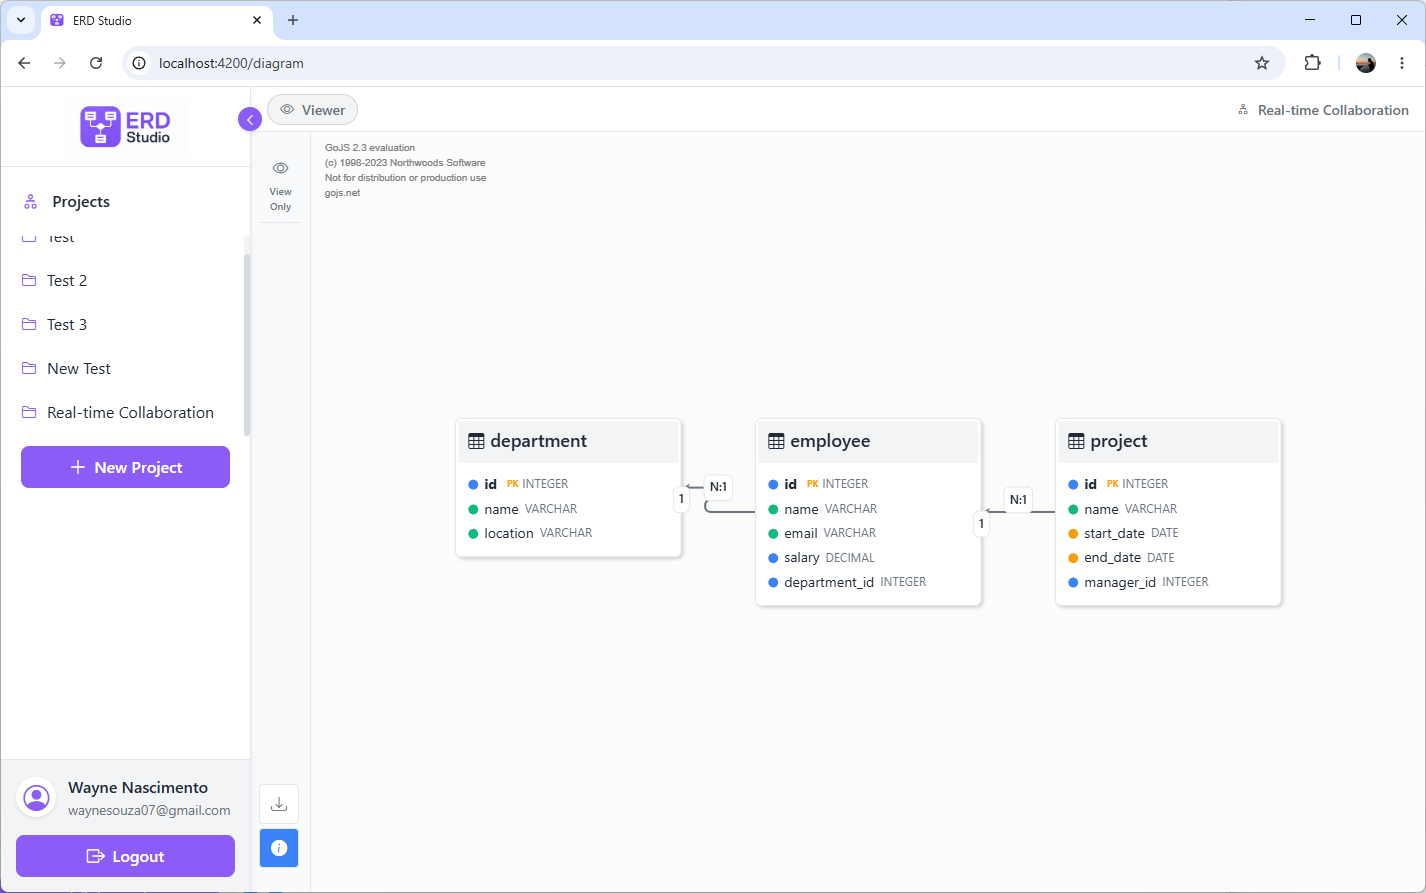
\includegraphics[width=15cm]{figuras/interface/tela-com-diagrama-simples-no-perfil-viewer.png}
    \caption{Editor de diagramas no perfil \textit{Viewer}}
    \begin{center}
        {\small Fonte: Elaborado pelo autor}
    \end{center}
    \label{fig:perfil-viewer}
\end{figure}

O mecanismo de bloqueio de entidades garante a consistência do diagrama durante sessões colaborativas simultâneas. Quando um colaborador inicia a edição de uma entidade, ela é bloqueada para os demais usuários conectados ao projeto. A Figura~\ref{fig:elemento-bloqueado} ilustra esse comportamento: a entidade \textit{employee} exibe uma borda tracejada indicando que está sendo editada por outro usuário, e uma notificação é exibida no topo da tela identificando o colaborador responsável pela edição.

\begin{figure}[H]
    \centering
    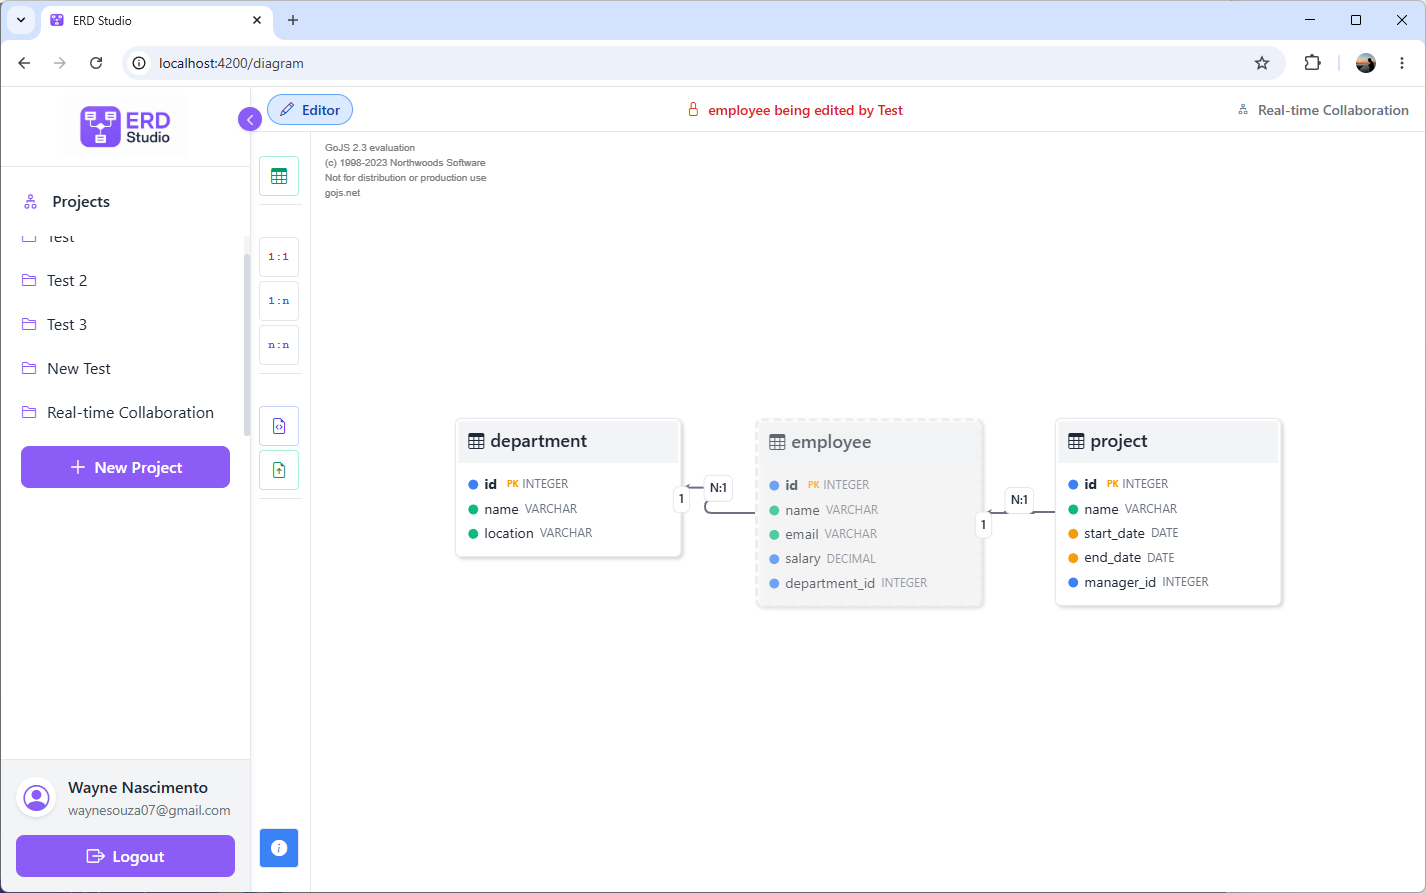
\includegraphics[width=15cm]{figuras/interface/tela-com-diagrama-simples-mostrando-elemento-bloqueado-por-outro-usuario.png}
    \caption{Entidade bloqueada por outro colaborador durante edição simultânea}
    \begin{center}
        {\small Fonte: Elaborado pelo autor}
    \end{center}
    \label{fig:elemento-bloqueado}
\end{figure}

\section{Disponibilidade do Código-Fonte e da Aplicação}

O código-fonte do protótipo está organizado em dois repositórios públicos no GitHub, separados por módulo:

\begin{itemize}
    \item \textbf{\textit{Back-end}:} \url{https://github.com/waynesouza/erd-core}
    \item \textbf{\textit{Front-end}:} \url{https://github.com/waynesouza/erd-client}
\end{itemize}

Após a implantação, a aplicação estará acessível temporariamente pelo navegador no seguinte endereço: \url{https://PLACEHOLDER_URL}. % TODO: substituir pela URL de deploy

% ----------------------------------------------------------
\chapter{Resultados e Discussões}
% ----------------------------------------------------------

Os resultados apresentados no capítulo anterior demonstram que o protótipo de modelador de diagramas ER colaborativo entregou um sistema funcional que integra modelagem de dados, colaboração em tempo real e controle de acesso em uma única plataforma \textit{web}. Este capítulo discute esses resultados sob duas perspectivas: a comparação com ferramentas estabelecidas no mercado e a análise das dificuldades encontradas e das limitações do protótipo.

% ----------------------------------------------------------
\section{Comparação com Ferramentas Existentes}
% ----------------------------------------------------------

A fim de contextualizar o protótipo desenvolvido, a Tabela~\ref{tab:comparacao} apresenta uma comparação entre o protótipo e três ferramentas de modelagem ER disponíveis no mercado: Lucidchart, DBdiagram.io e MySQL Workbench.

\begin{table}[H]
\centering
\caption{Comparação entre o protótipo e ferramentas de modelagem ER}
\label{tab:comparacao}
\begin{tabular}{|l|c|c|c|c|}
\hline
\textbf{Funcionalidade} & \textbf{Protótipo} & \textbf{Lucidchart} & \textbf{DBdiagram.io} & \textbf{MySQL Workbench} \\
\hline
Modelagem ER              & Sim    & Sim      & Sim      & Sim \\
\hline
Colaboração em tempo real & Sim    & Pago     & Não      & Não \\
\hline
Exportação DDL (SQL)      & Sim    & Pago     & Sim      & Sim \\
\hline
Importação DDL (SQL)      & Sim    & Não      & Sim      & Sim \\
\hline
Baseado em \textit{web}   & Sim    & Sim      & Sim      & Não \\
\hline
Gratuito                  & Sim    & Parcial  & Parcial  & Sim \\
\hline
\end{tabular}
\begin{center}
    {\small Fonte: Elaborado pelo autor}
\end{center}
\end{table}

A análise comparativa evidencia que o protótipo desenvolvido distingue-se por reunir, em uma plataforma \textit{web} e de forma gratuita, as funcionalidades de colaboração em tempo real e de importação e exportação DDL. O Lucidchart, embora ofereça colaboração em tempo real, restringe esse recurso a planos pagos. O MySQL Workbench, apesar de robusto na modelagem e no suporte DDL, opera como uma aplicação \textit{desktop} e não oferece colaboração entre usuários. O DBdiagram.io, por sua vez, oferece suporte a DDL, mas carece da funcionalidade colaborativa. O protótipo preenche a intersecção dessas capacidades, alinhando-se ao diagnóstico de lacuna identificado na justificativa do trabalho: a ausência de uma ferramenta \textit{web}, acessível e colaborativa para a modelagem de diagramas ER.

% ----------------------------------------------------------
\section{Dificuldades e Lições Aprendidas}
% ----------------------------------------------------------

O desenvolvimento do protótipo apresentou desafios técnicos relevantes. A sincronização do estado do diagrama em um cenário de múltiplos colaboradores simultâneos constituiu a maior complexidade do projeto. A garantia de consistência --- propagando alterações de forma ordenada e prevenindo conflitos sem introduzir latência perceptível ao usuário --- exigiu iterações de projeto sobre a estratégia de \textit{locks} em memória e sobre a estrutura de mensagens STOMP. O modelo de \textit{locks} com \textit{timeout} automático demonstrou ser uma solução pragmática e suficiente para o escopo do protótipo.

A integração da biblioteca GoJS com o mecanismo de detecção de mudanças do Angular também demandou atenção. Alterações no modelo do diagrama originadas externamente, via WebSocket, precisaram ser aplicadas ao canvas da GoJS de maneira a não disparar ciclos redundantes de atualização, o que exigiu controle explícito das zonas de execução do Angular.

Por fim, a adoção da persistência poliglota --- PostgreSQL e MongoDB --- conferiu flexibilidade ao modelo de dados e desempenho adequado a cada tipo de operação. No entanto, essa decisão impôs a necessidade de gerenciar dois sistemas de banco de dados distintos, tanto no ambiente de desenvolvimento local quanto na configuração do Docker Compose para implantação, aumentando a complexidade operacional do projeto.

% ----------------------------------------------------------
\section{Limitações do Protótipo}
% ----------------------------------------------------------

Apesar dos resultados alcançados, o protótipo apresenta limitações que definem seu escopo em relação a uma solução de produção.

A primeira limitação refere-se à \textbf{ausência de um histórico de versões do diagrama}. Na versão atual, o estado do diagrama é substituído a cada atualização persistida, sem preservação de versões anteriores. Isso impede que os colaboradores desfaçam alterações em nível colaborativo ou inspecionem o histórico de mudanças do projeto, funcionalidade presente em ferramentas maduras de colaboração. A implementação de um mecanismo de versionamento, como o armazenamento de \textit{snapshots} incrementais, constitui uma evolução natural do protótipo.

A segunda limitação diz respeito à \textbf{licença comercial da biblioteca GoJS}. A GoJS exige a aquisição de uma licença para uso em ambiente de produção, disponibilizando apenas uma licença de avaliação para fins acadêmicos e de prototipagem. A adoção do protótipo em contexto comercial estaria sujeita a esses custos de licenciamento. Em trabalhos futuros, a substituição da GoJS por uma alternativa de código aberto com capacidades equivalentes seria um caminho viável para eliminar essa restrição.

% ----------------------------------------------------------
\chapter{Considerações Finais}
% ----------------------------------------------------------

O presente trabalho cumpriu com seus objetivos, demonstrando a viabilidade de desenvolver um protótipo de modelador de diagramas ER colaborativo acessível via navegador. A plataforma resultante integra, em uma única solução gratuita, a modelagem interativa de esquemas de banco de dados, a colaboração em tempo real entre múltiplos usuários e operações de importação e exportação DDL, conjunto de capacidades que, conforme evidenciado na comparação com ferramentas do mercado, não encontra equivalente gratuito disponível.

Os cinco objetivos específicos definidos na introdução foram atendidos. O primeiro objetivo, referente à modelagem e persistência dos elementos do diagrama, foi atendido pelo editor interativo desenvolvido, que captura entidades, atributos, relacionamentos, tipos de dados e posicionamentos, preservando o estado completo do diagrama. O segundo objetivo, de investigar a principal biblioteca de diagramação adotada, foi cumprido ao longo do desenvolvimento: a biblioteca demonstrou-se adequada para a renderização interativa de diagramas ER e para a aplicação de atualizações provenientes de outros colaboradores em tempo real. O terceiro objetivo, de permitir a colaboração simultânea de múltiplos usuários, foi alcançado por meio de comunicação bidirecional em tempo real, com mecanismo de controle de acesso por entidade para prevenção de conflitos. O quarto objetivo, de implementar autenticação e autorização, foi satisfeito pela combinação de mecanismos de segurança no servidor e no cliente. O quinto objetivo, de adotar práticas ágeis, foi contemplado pela aplicação adaptada de metodologia ágil com acompanhamento visual do progresso durante todo o ciclo de desenvolvimento.

O ganho proporcionado por este trabalho se manifesta em duas dimensões. Do ponto de vista técnico, o protótipo serve como referência prática para a construção de ferramentas colaborativas baseadas em comunicação em tempo real com editores visuais interativos em ambiente \textit{web}. Do ponto de vista da área, o trabalho contribui para preencher a lacuna identificada na justificativa: a carência de uma ferramenta colaborativa, baseada em \textit{web} e sem barreiras de custo para a modelagem de diagramas ER, atendendo às demandas de equipes de desenvolvimento distribuídas.

% % ----------------------------------------------------------
\chapter{Cronograma}
% ----------------------------------------------------------

Na tabela \ref{tab:cronograma} apresentada abaixo, as tarefas estão distribuídas ao longo de dois períodos distintos. As atividades enumeradas de 1 a 5 estão programadas para o período compreendido entre agosto e dezembro de 2023. Por outro lado, as tarefas de 6 a 11 estão agendadas para serem executadas no semestre que se estende de janeiro a junho de 2024. As tarefas são divididas do seguinte modo:

\begin{enumerate}
  \item \textbf{Definição do escopo e fluxos}: Esta fase envolve a definição clara do escopo do projeto e a identificação dos fluxos de trabalho necessários.
  \item \textbf{Implementação}: Nesta fase, a implementação real do projeto ocorre, com base no escopo e nos fluxos definidos anteriormente.
  \item \textbf{Documentação do código}: Aqui, a documentação detalhada do código desenvolvido é criada, facilitando a manutenção e a compreensão futura.
  \item \textbf{Deploy e testes}: O código é implantado em um ambiente e serão realizados testes extensivos para garantir que tudo está funcionando como esperado.
\end{enumerate}

\begin{table}[h]
\centering
\begin{tabular}{r*{11}{|c}|}
\cline{2-12} 
 & \multicolumn{11}{c|}{2023/2024} \\
\cline{2-12}
 & 1 & 2 & 3 & 4 & 5 & 6 & 7 & 8 & 9 & 10 & 11 \\
\cline{2-12}
\textbf{Definição} & X & X & X &   &   &   &   &   &   &   &   \\
\cline{2-12}
Atividade 1 & X & X & X &   &   &   &   &   &   &   &   \\
\cline{2-12}
\textbf{Implementação} &   &   & X & X & X & X & X & X & X &   &   \\
\cline{2-12}
Atividade 2 &   &   & X & X & X & X & X & X &   &   &   \\
\cline{2-12}
Atividade 3 &   &   &   &   &   &   & X & X & X &   &   \\
\cline{2-12}
Atividade 4 &   &   &   &   &   &   &   & X & X &   &   \\
\cline{2-12}
\textbf{Monografia} &   &   &   &   &   &   & X & X & X & X & X \\
\cline{2-12}
Escrita &   &   &   &   &   &   & X & X & X & X &   \\
\cline{2-12}
Defesa &   &   &   &   &   &   &   &   &   & X & X \\
\cline{2-12}
\end{tabular}
\caption{Cronograma das atividades do projeto}
\label{tab:cronograma}
\end{table}

% ----------------------------------------------------------
\chapter{Resultados Esperados}
% ----------------------------------------------------------

O objetivo do projeto Protótipo de um modelador de diagramas ER colaborativo é fornecer uma ferramenta capaz e acessível que atenda às demandas atuais de projetos de TI. Ao fornecer uma solução que simplifica de forma eficaz e colaborativa a modelagem de diagramas ER, esta iniciativa deve preencher uma lacuna significativa no mercado. A ferramenta em desenvolvimento promove a troca de ideias mais eficaz e a resolução de problemas em grupo.

Ademais, o projeto aspira fomentar um ambiente laboral mais produtivo, salientando a eficácia e reduzindo os custos vinculados ao desenvolvimento de projetos de banco de dados. Por meio da promoção da colaboração em tempo real, espera-se que a ferramenta atenue atrasos e retrabalhos, contribuindo para um ciclo de desenvolvimento mais ágil e dinâmico. Este empreendimento não apenas atende às demandas de um mundo digital e interconectado, mas também se posiciona como um catalisador para futuras inovações tecnológicas no campo da TI.

Ao final deste projeto, espera-se que o protótipo criado se torne uma ferramenta útil, ajudando a modelar bancos de dados e promovendo a cooperação e a eficiência no desenvolvimento de projetos de TI.
% % ----------------------------------------------------------
\chapter{Trabalhos futuros}
% ----------------------------------------------------------

\chapter{Cronograma}


\phantompart

% ----------------------------------------------------------
% ELEMENTOS PÓS-TEXTUAIS
% ----------------------------------------------------------
\postextual

% Referências bibliográficas
\bibliography{monografia}

% \nocite{fds2017, LARAVEL2008, HTMLeCSS2008, AplicacaodePHP2007,  PHPPOO2015, PHPConhece2017, PHPMYSQL2011, JAVASCRIPTGuia2002}

% Consulte o manual da classe abntex2 para orientações 
% sobre os seguintes tópicos opcionais:

%------------ Glossário

%------------ Apêndices

%------------ Anexos
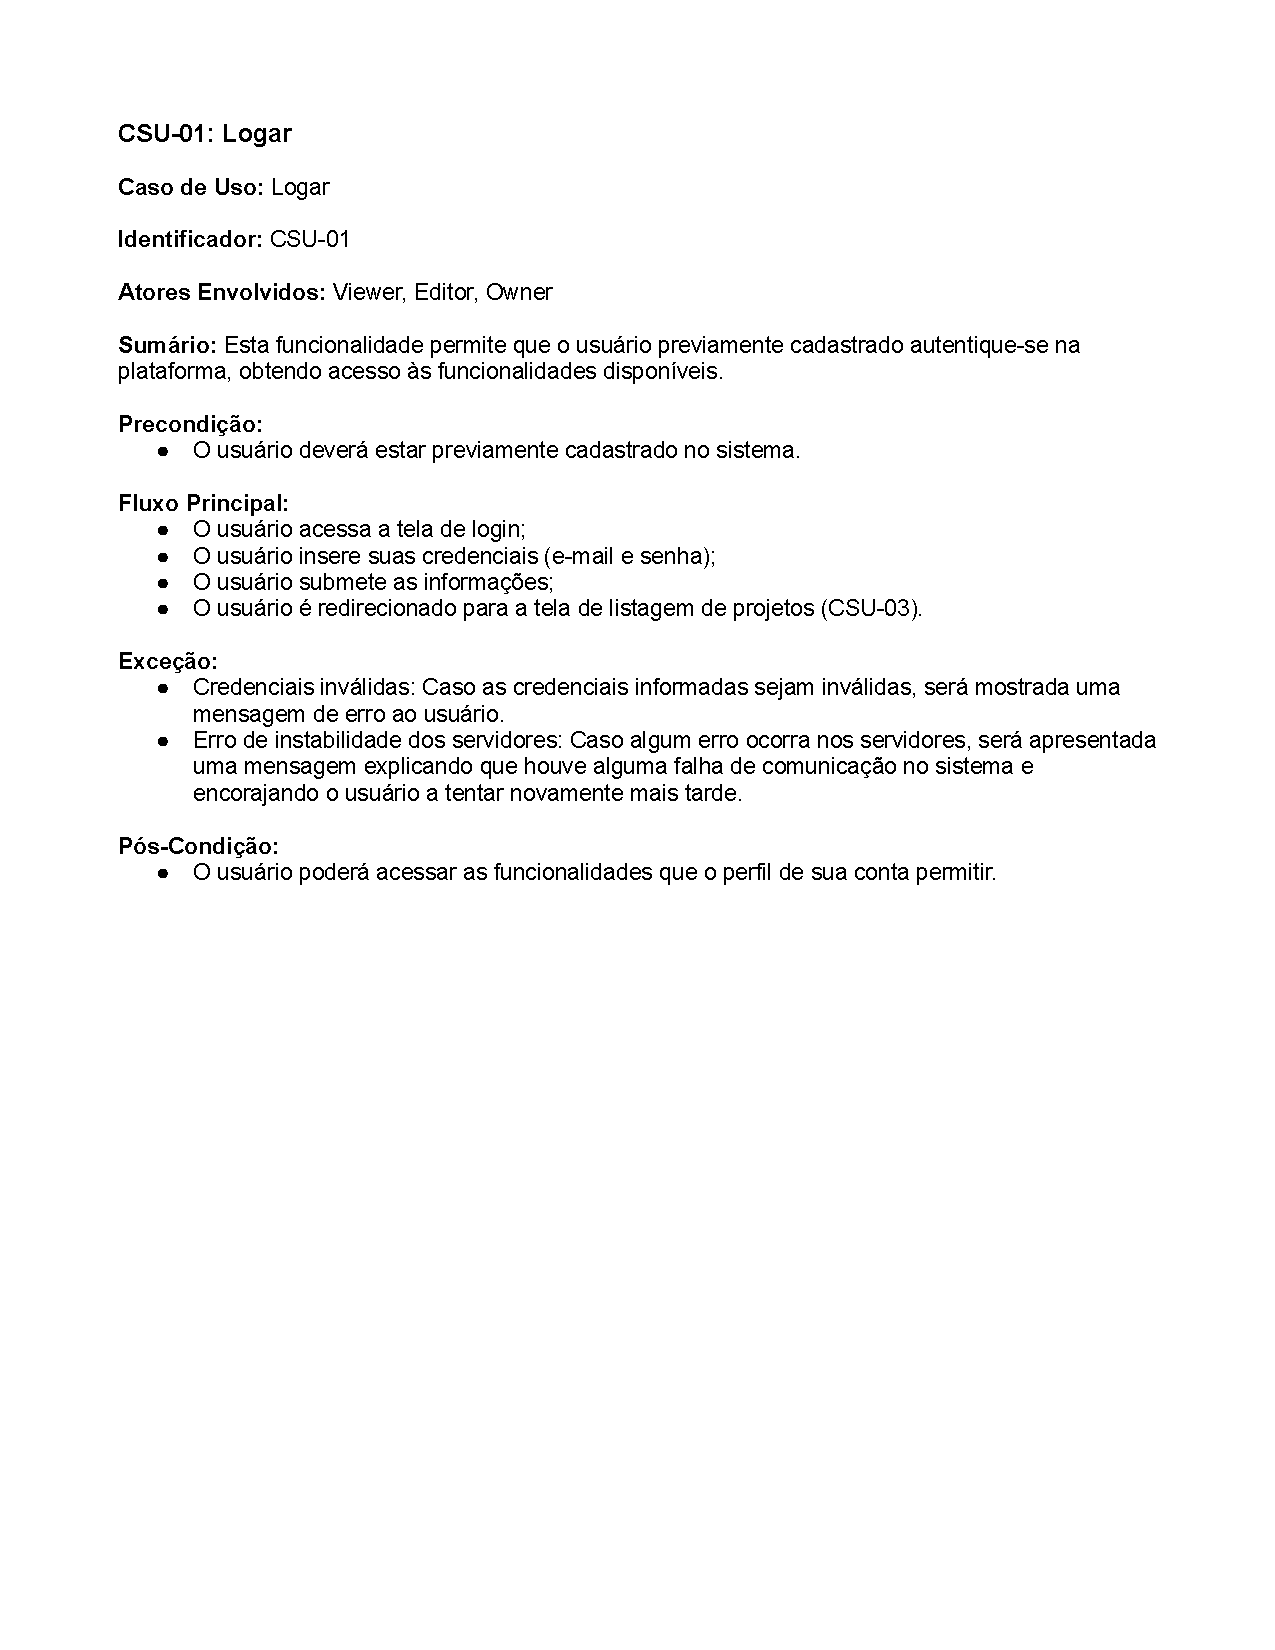
\includepdf[pages=-]{anexos/Expansão de Caso de Uso.pdf}

% INDICE REMISSIVO
\phantompart
\printindex

\end{document}
\grid
